\documentclass[]{politex}
% ========== Opções ==========
% pnumromarab - Numeração de páginas usando algarismos romanos na parte pré-textual e arábicos na parte textual
% abnttoc - Forçar paginação no sumário conforme ABNT (inclui "p." na frente das páginas)
% normalnum - Numeração contínua de figuras e tabelas 
%	(caso contrário, a numeração é reiniciada a cada capítulo)
\label{key}% draftprint - Ajusta as margens para impressão de rascunhos
%	(reduz a margem interna)
% twosideprint - Ajusta as margens para impressão frente e verso
% capsec - Forçar letras maiúsculas no título das seções
% espacosimples - Documento usando espaçamento simples
% espacoduplo - Documento usando espaçamento duplo
%	(o padrão é usar espaçamento 1.5)
% times - Tenta usar a fonte Times New Roman para o corpo do texto
% noindentfirst - Não indenta o primeiro parágrafo dos capítulos/seções
% ========== Opções do documento ==========
% Título
\titulo{VALIDAÇÃO DE ALGORITMOS DE FOTOPLETISMOGRAFIA REMOTA PARA ESTIMATIVA DE SINAIS VITAIS DE PACIENTES EM UNIDADES DE TERAPIA INTENSIVA}
% \versao{0}
% Autor
\autor{Sophia Celine Rafael Alves Pereira}

% Para múltiplos autores (TCC)
%\autor{Nome Sobrenome\\%
%		Nome Sobrenome\\%
%		Nome Sobrenome}

% Orientador / Coorientador
\orientador{Dr. Felipe Fava de Lima}

%\coorientador{Nome do coorientador (opcional)}

% Tipo de documento
%\tcc{Engenheiro Civil}
% \dissertacao{Ciências}
\qualificacao{Ciências}
%\teseDOC{Engenharia Transportes}
%\teseLD
%\memorialLD

% Departamento e área de concentração
\departamento{Departamento de Engenharia de Telecomunicações e Controle}
\areaConcentracao{Engenharia Biomédica}

% Local
\local{São Paulo}

% Ano
\data{2026}

\begin{document}
% ========== Capa e folhas de rosto ==========
\capa
%\falsafolhaderosto
% \folhaderosto
% ========== Ficha catalográfica ==========
% Fazer solicitação no site:
%	http://www.poli.usp.br/en/bibliotecas/servicos/catalogacao-na-publicacao.html

%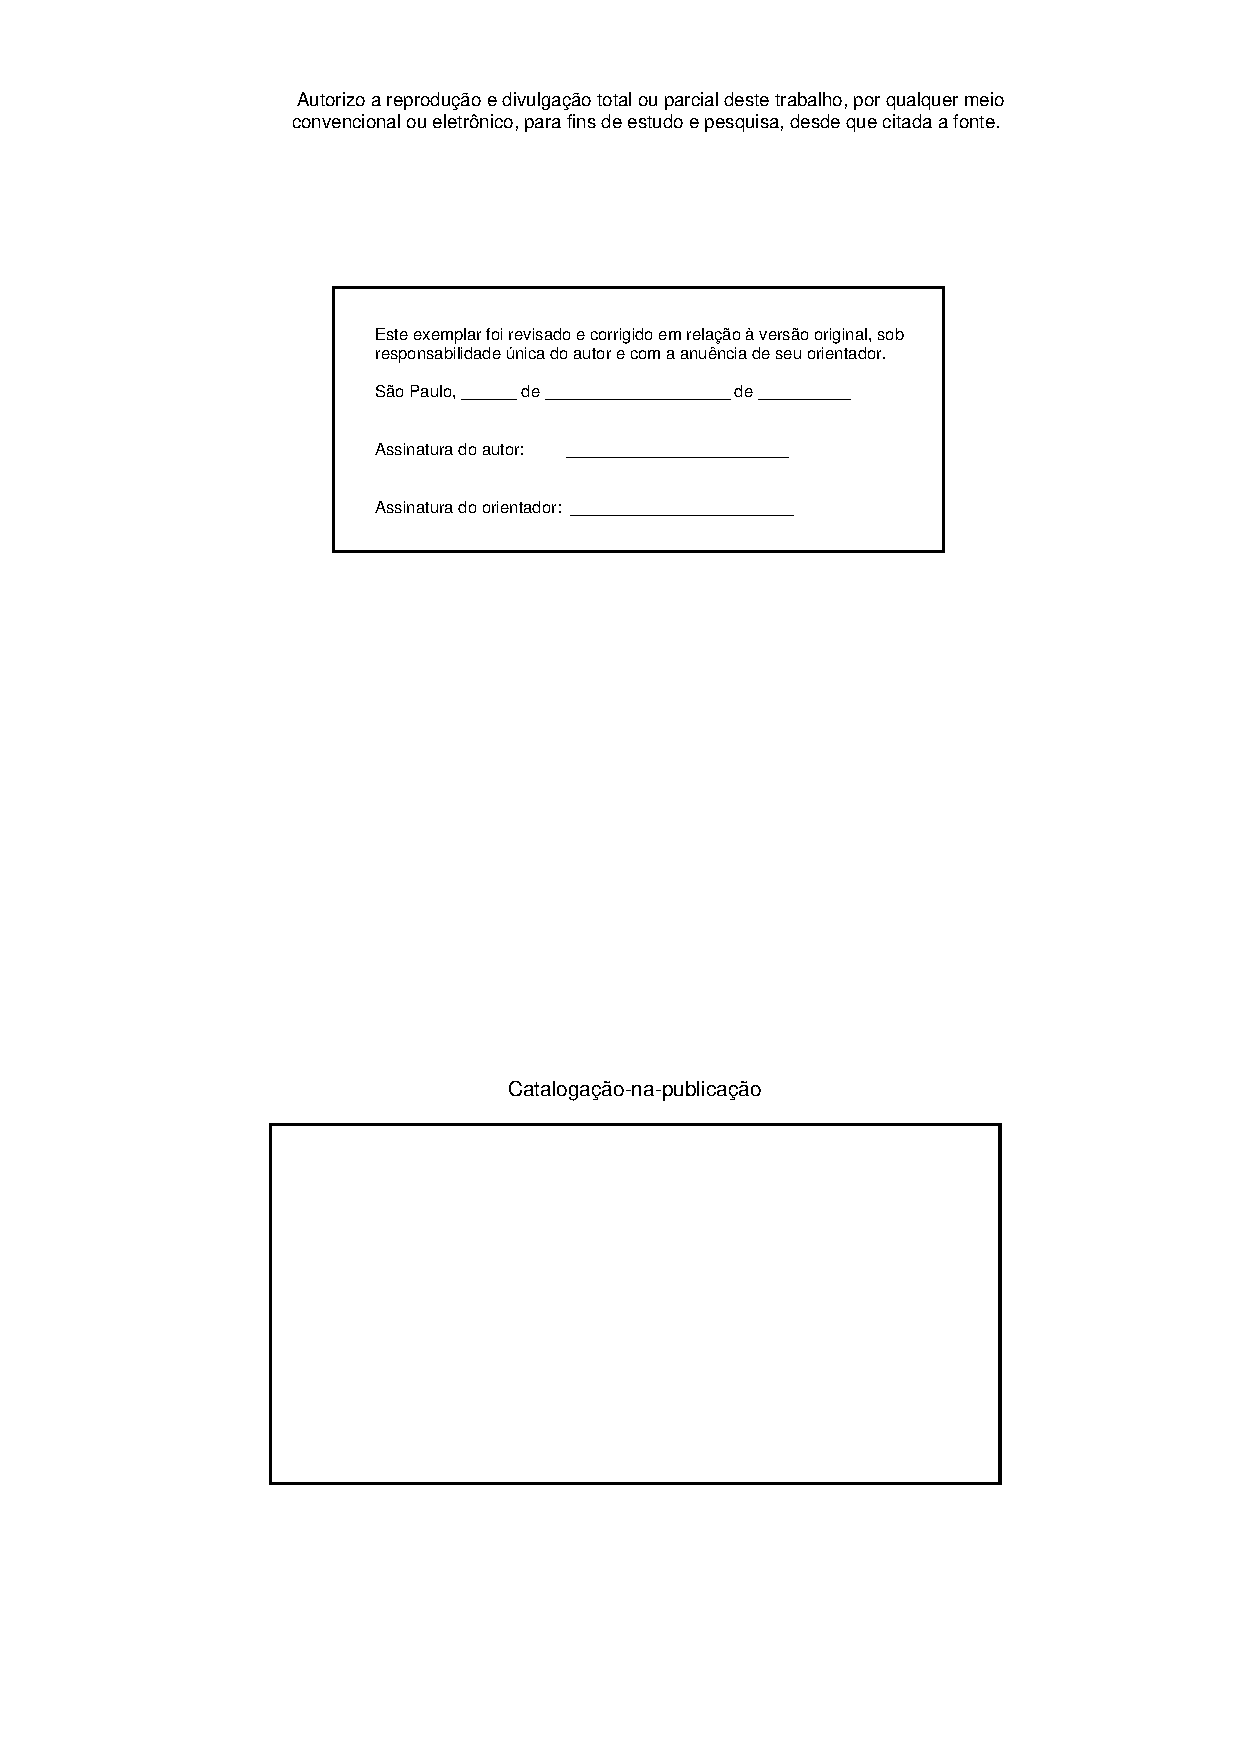
\includepdf[pages=1,scale=1,pagecommand={},%linktodoc=true]{ficha.pdf}
% ========== Folha de assinaturas (opcional) ==========
%\begin{folhadeaprovacao}
%	\assinatura{Orientador}
%	\assinatura{Avaliador 1}
%	\assinatura{Avaliador 2}
%\end{folhadeaprovacao}


% ========== Dedicatória (opcional) ==========
%\dedicatoria{À minha mãe, que me mostrou a beleza da ciência. Ao meu pai, que me ensinou a aprender o mundo. E a todos os meus professores que, com seu próprio brilho no olhar, iluminaram meu caminho de descobertas.}

% ========== Agradecimentos ==========
%\begin{agradecimentos}

%ao meu orientador, ao HU, ao Paolo do HU, aos meus pais

%\end{agradecimentos}


% ========== Epígrafe (opcional) ==========
%\epigrafe{%
%	\emph{``Epígrafe''}
%	\begin{flushright}
%		\blindtext
%	\end{flushright}
%}


% ========== Resumo ==========
\begin{resumo}
O monitoramento de sinais vitais é fundamental para a avaliação do estado fisiológico de pacientes e, tradicionalmente, é realizado por meio de dispositivos médicos de contato. Entretanto, abordagens de monitoramento não invasivo apresentam benefícios relevantes, tanto em contextos clínicos quanto não clínicos, ao possibilitarem maior conforto ao paciente, redução de riscos associados ao contato físico e maior flexibilidade de aplicação. Nesse contexto, a fotopletismografia remota (rPPG) destaca-se como uma abordagem promissora para a estimativa de parâmetros fisiológicos, como frequência cardíaca e respiratória, saturação de oxigênio e pressão arterial, a partir da detecção de variações cíclicas do sistema cardiovascular que podem ser extraídas a partir das mudanças sutis de intensidade dos elementos de cor de regiões da pele captadas por vídeo. Embora existam diversos métodos, tanto não supervisionados quanto baseados em aprendizado profundo, a maioria dos estudos é conduzida em cenários controlados, envolvendo predominantemente indivíduos saudáveis. Diante dessa limitação, este trabalho busca analisar o desempenho dos principais algoritmos de rPPG em vídeos de pacientes de uma Unidade de Terapia Intensiva (UTI) inserida no contexto do Sistema Único de Saúde (SUS) brasileiro. Ademais, propõe-se a construção de uma base de dados específica para esse cenário, composta por vídeos adquiridos por uma câmera de vídeo industrial e por sinais de referência obtidos diretamente de monitores multiparâmetros hospitalares. Por fim, os resultados visam avaliar a robustez e a viabilidade clínica dos métodos de rPPG em condições reais de cuidados intensivos.
%
\\[3\baselineskip]
%
\textbf{Palavras-Chave} fotopletismografia remota, unidade de terapia intensiva, sinais vitais.
\end{resumo}

% ========== Abstract ==========
\begin{abstract}
Vital sign monitoring is essential for evaluating the physiological state of a patient and is typically performed using contact-based medical devices. Nonetheless, non-invasive monitoring approaches offer relevant benefits in both clinical and non-clinical settings by increasing patient comfort, reducing contact-associated risks, and providing greater flexibility of application. In this context, remote photoplethysmography (rPPG) has emerged as a promising technique for estimating physiological parameters such as heart rate, respiratory rate, oxygen saturation and blood pressure by detecting cyclical variations of the cardiovascular system which can be extracted from sutil changes in the color intensity of pixels from the skin region captured by video. Although several methods have been proposed, including unsupervised approaches and deep learning–based techniques, most studies are conducted under controlled conditions and involve predominantly healthy individuals. In view of this limitation, this work aims to assess the performance of the main rPPG algorithms using video recordings of patients in a public Intensive Care Unit (ICU) which is part of the brazilian Unified Health System (Sistema Único de Saúde - SUS). In addition, a new dataset specific to this context is proposed, comprising video recordings acquired using an industrial video camera and reference signals collected directly from hospital multiparameter monitors. The results aim to assess the robustness and clinical feasibility of rPPG methods under realistic intensive care conditions. 
%
\\[3\baselineskip]
%
\textbf{Keywords} remote photopletysmography, intensive care unit, vital signs.
\end{abstract}

% ========== Listas (opcional) ==========
\listadefiguras
\listadetabelas

% ========== Listas definidas pelo usuário (opcional) ==========
% \newpage\begin{pretextualsection}{Lista de Abreviações}

\noindent
rPPG – \textit{remote photopletismography} (fotopletismografia remota)\\
PPG - \textit{photopletismography} (fotopletismografia) \\
UTI - Unidade de Terapia Intensiva \\
UTIN - Unidade de Terapia Intensiva Neonatal \\
ROI - \textit{region of interest} (região de interesse) \\
DL - \textit{deep learning} (aprendizado profundo) \\
ECG - eletrocardiograma \\
FFT - Transformada Rápida de Fourier \\
BSS - \textit{blind source separation} (separação cega de sinais) \\
ICA - Análise de Componentes Independentes \\
PCA - Análise de Componentes Principais \\

\end{pretextualsection}

% ========== Sumário ==========
\sumario

% ========== Elementos textuais =======

\newpage\chapter{Introdução}
\label{intro}

A medição de sinais vitais é uma prática essencial para a avaliação das condições fisiológicas de um indivíduo e para garantir tratamentos adequados e evitar a deterioração de condições de saúde que podem ser prevenidas \cite{elliott2012vitalsigns}. Por esse motivo, no cenário clínico, especialmente no cuidado de pacientes de alto risco, há monitoramento contínuo com o uso de equipamentos médicos automatizados, a fim de possibilitar que mudanças significativas nos parâmetros fisiológicos possam ser prontamente identificadas e tratadas. A título de exemplo, a função cardíaca é tipicamente monitorada com o uso do eletrocardiograma (ECG), assim como a saturação de oxigênio é avaliada com o uso de oxímetros de pulso e a frequência respiratória é monitorada por pneumografia por impedância, que comumente utiliza os mesmos eletrodos que os equipamentos de ECG. 

No entanto, as restrições impostas pelo monitoramento contínuo por dispositivos com fios e contato direto com o corpo, principalmente durante períodos prolongados, podem gerar incômodo e são consideradas um dos fatores mais citados como agentes estressores para pacientes em Unidades de Terapia Intensiva (UTIs) \cite{ede2021ICUhumanfactors}. De fato, no contexto de Unidades de Terapia Intensiva Neonatal (UTINs), os dispositivos de medição requerem sensores adesivos que podem ocasionar lesões em recém-nascidos prematuros, os quais possuem a pele frágil, além de causar dor. Em contrapartida, soluções de medição de frequência cardíaca (FC), frequência respiratória (FR) e saturação de oxigênio  por câmera mostram acurácia clinicamente significativa e comparável aos métodos tradicionais nesse cenário \cite{villarroel2014neonatal}. 

Ademais, o monitoramento em UTIs apresenta desafios sobretudo durante o transporte de pacientes e devido ao mau contato dos sensores ou à má qualidade do sinal. Nesse caso, a monitorização por câmera se mostra uma alternativa capaz fornecer estimativas confiáveis das frequências cardíaca e respiratória e, principalmente, prever alterações no ritmo respiratório de forma condizente com o estado fisiológico em situações nas quais a aquisição por equipamentos de contato está ausente. Além disso, esse tipo de solução complementa essas medições e pode oferecer informações visuais sobre a morfologia do esforço respiratório e evidenciar assimetrias que contribuem para o diagnóstico de condições clínicas \cite{jorge2022postOpICU}.

A partir disso, diante dos desafios impostos pela aquisição de sinais vitais por meio de equipamentos médicos de contato, a medição de parâmetros fisiológicos por câmera apresenta-se como uma estratégia confiável e possui vantagens de custo e facilidade de aplicação comparado a outras estratégias de monitorização remota, como as baseadas em indução magnética, efeito Doppler ou imageamento térmico \cite{khanam2019clinicalnonclinicalReview}. Nesse sentido, as soluções de medição por câmera baseiam-se, principalmente, em métodos de fotopletismografia remota (rPPG), os quais possuem o objetivo de detectar as variações cíclicas do sistema cardiovascular que podem ser extraídas a partir das mudanças sutis de intensidade dos elementos de cor de uma área do corpo ao longo do tempo. Assim, a luz que é re-emitida após passar pelos tecidos da pele é captada por dispositivos de aquisição de imagens, sendo que as propriedades óticas da superfície do corpo são influenciadas sobretudo pela hemoglobina e pela melanina da região analisada. Em função das características descritas, as principais aplicações utilizam não só câmeras RGB convencionais, mas também câmeras sensíveis ao infravermelho ou ao infravermelho próximo \cite{selvaraju2022continuous}.

Dessa forma, a compreensão detalhada da fotopletismografia remota requer, inicialmente, a definição dos princípios básicos da fotopletismografia (PPG). A PPG é uma técnica ótica de medição que pode ser utilizada para detectar variações no volume sanguíneo no leito microvascular dos tecidos. Desse modo, o sinal característico dessa técnica possui uma componente pulsátil chamada de componente AC com frequência fundamental próxima a 1 Hz e que depende do batimento cardíaco, conforme ilustra a Figura \ref{fig:ppgWave}. Analogamente, há uma componente DC que varia lentamente de acordo com a respiração, com a atividade vasomotora e com ondas vasoconstritoras, além de ondas Traube-Hering-Mayer (THM) relativas a oscilações da pressão arterial. Esse sinal pode ser percebido devido às características óticas da pele, sendo que os fatores primordiais que afetam a quantidade de luz recebida por um fotodetector de um tecido iluminado são o volume sanguíneo, a movimentação das paredes dos vasos e a orientação das células vermelhas. Há, ainda a influência do comprimento de onda da fonte na interação entre a pele e a luz, de modo que a medição convencional desse sinal, tipicamente realizada por oxímetros de pulso, utiliza feixes na faixa do vermelho e do infravermelho para detecção da saturação periférica de oxigênio baseada nas propriedades óticas de absorção da oxihemoglobina e da desoxihemoglobina nessas regiões do espectro eletromagnético \cite{allen2007photoplethysmography}.

\begin{figure}[H]
    \centering
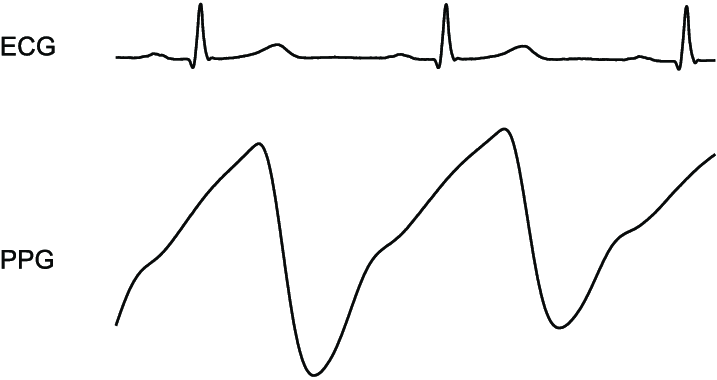
\includegraphics[width=0.6\linewidth]{imagens/PPGwaveAllen2007.png}
    \caption{Componente pulsátil do sinal de PPG e o ECG correspondente} 
    Fonte: \citeonline{allen2007photoplethysmography}
    \label{fig:ppgWave}
\end{figure}

Diante do exposto, a literatura mostra que é possível obter um sinal de PPG de forma remota com o uso de câmeras convencionais e utilizando a luz ambiente como principal fonte de iluminação, por meio da análise das variações dos canais de cor de regiões de interesse específicas \cite{verkruysse2008remote}. Além disso, a fim de definir princípios bem estabelecidos para a extração de sinais de rPPG, os principais métodos consideram a modelagem da interação entre a luz e a pele com base na lei de Beer-Lambert, a qual descreve como a absorção da luz por uma substância depende de sua concentração e do caminho percorrido pelo feixe, ou no modelo dicromático de reflexão de Shafer, o qual define que a luz refletida por um material dielétrico não homogêneo pode ser dividida em uma componente de reflexão difusa e uma componente de reflexão especular \cite{chen2018deepphys}.

Nesse contexto, a extração do sinal de rPPG pode ser realizada tanto com o uso exclusivo de luz ambiente quanto por meio de fontes de iluminação controladas, com um ou mais dispositivos de aquisição de imagens para a captura de dados de vídeo \cite{mcduff2015survey}. A metodologia usual envolve a detecção e o rastreamento de uma região de interesse (ROI), a partir da qual é obtido o sinal bruto por meio da análise dos canais de cor dos pixeis de cada frame. Posteriormente, esse sinal é filtrado e processado a fim de reconstruir a onda de pulso de volume sanguíneo (BVP) característica da fotopletismografia, cujas propriedades podem ser utilizadas para a estimação de parâmetros fisiológicos \cite{rouast2018review}, conforme esquematiza a Figura \ref{fig:rppgschematic}.

\begin{figure}[H]
    \centering
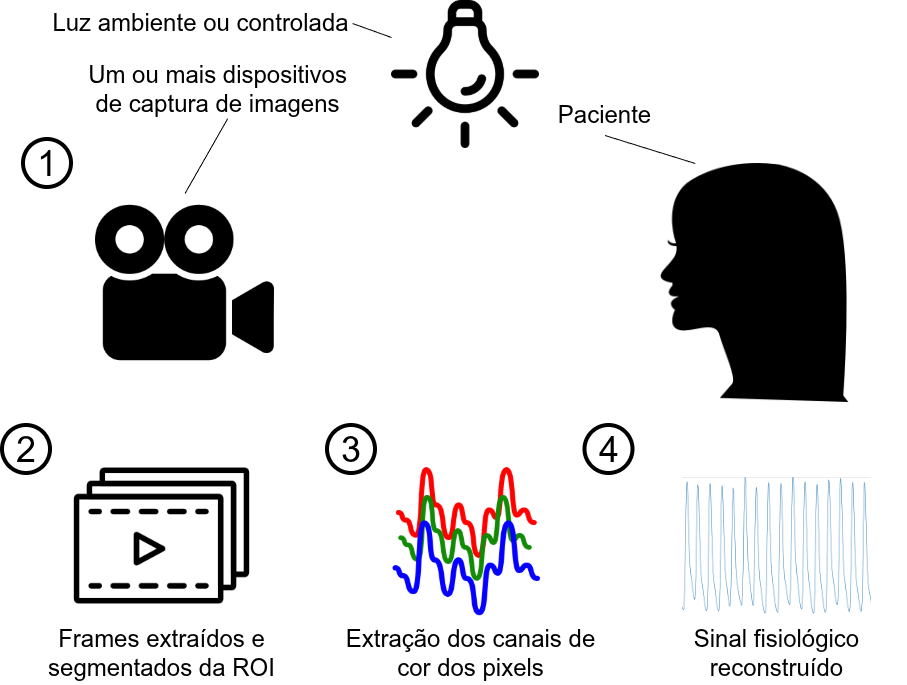
\includegraphics[width=0.6\linewidth]{imagens/rPPGschematic.png}
    \caption{Esquemático da extração de sinais por fotopletismografia remota} 
    Fonte: Adaptado de \citeonline{mcduff2015survey}
    \label{fig:rppgschematic}
\end{figure}

Por conseguinte, as principais implementações utilizam métodos não supervisionados, bem como métodos baseados em aprendizado profundo (\textit{deep learning}, DL). Os métodos não supervisionados extraem os sinais fisiológicos por estratégias de análise de cor ou de movimento das imagens de entrada. Sistemas baseados em DL, por sua vez, utilizam tanto modelos fim a fim, os quais são treinados para extraírem o sinal de rPPG ou diretamente parâmetros fisiológicos a partir de dados de vídeo como entrada, quanto sistemas híbridos, os quais combinam métodos algorítmicos com modelos de DL que extraem características específicas em uma ou mais partes do processo de estimação de parâmetros. Desse modo, pode-se extrair dados de perfusão sanguínea periférica, frequência respiratória, saturação de oxigênio, frequência cardíaca e de pulso, variabilidade das frequências cardíaca e de pulso e pressão arterial por meio das diferentes abordagens \cite{chen2024deep}.
 
 Em vista disso, a extração do sinal de rPPG possui crescente potencial de aplicabilidade, por exemplo, no monitoramento dos parâmetros fisiológicos de pacientes em sessões de tratamento de hemodiálise. Nesse cenário, algoritmos de imageamento fotopletismográfico podem estimar valores de frequência cardíaca com boa concordância em relação aos adquiridos por equipamentos médicos de referência \cite{villarroel2017non, villarroel2020non}. Adicionalmente, nesse mesmo contexto clínico, os sinais de frequência respiratória adquiridos por esses métodos podem ser considerados mais estáveis que os obtidos com a utilização de cintas torácicas \cite{tarassenko2014non}. 
 
 Outro tipo de aplicação envolve a detecção de fibrilação atrial com base no sinal de fotopletismografia obtido remotamente. Para isso, é possível analisar índices estatísticos de variabilidade da frequência cardíaca baseados no pulso extraído dos dados de vídeo dos indivíduos analisados \cite{couderc2015detection}. Ademais, pode-se utilizar modelos de aprendizado profundo para classificar os sinais de rPPG de pacientes, de modo a indicar se possuem essa condição, se possuem ritmo sinusal normal ou outros tipos de alterações no ritmo cardíaco \cite{sun2022contactless}.

Observa-se, ainda, que a medição de sinais vitais de forma remota possui relevância no contexto de missões de busca e resgate para triagem de vítimas, sendo que há implementações que envolvem a aquisição de vídeos por câmeras embarcadas em veículos aéreos não tripulados. A partir dessas imagens, é possível extrair sinais de frequência cardíaca e respiratória com boa concordância em relação a dispositivos de referência como transdutores piezoelétricos de cinta respiratória e oxímetros de pulso. Nesse caso, a utilização de algoritmos de redução de ruídos é essencial para minimizar a influência de variações de iluminação e da movimentação tanto da câmera quanto dos indivíduos monitorados \cite{al2017remote}.

De modo complementar, a fotopletismografia remota possui potencial de aplicação para disparo cardíaco em procedimentos de ressonância magnética. A obtenção da onda de rPPG pode ser utilizada para iniciar a captura de imagens em momentos específicos do ciclo cardíaco. Esse tipo de abordagem, sobretudo na aquisição realizada por equipamentos de campo ultra-alto, evita o contato físico e possui menor interferência de artefatos em relação à oximetria de pulso e ao eletrocardiograma, que são os principais métodos de contato utilizados nesse contexto \cite{spicher2016initial}. 

O monitoramento remoto de parâmetros fisiológicos apresenta, adicionalmente, vantagens em relação a abordagens convencionais sobretudo no que se refere à realização de exercícios físicos, em que a medição por contato é dificultada \cite{napolean2022heart}. Durante a prática esportiva, as frequências cardíaca e respiratória são importantes para o cálculo do índice de intensidade de atividade física o qual, por sua vez, possibilita uma análise do esforço realizado. Assim, é possível evitar lesões por meio da identificação de condições de fadiga extrema a partir desse índice, que pode ser obtido com base nos sinais extraídos por câmera \cite{wu2023motion}. 

Com base nas discussões apresentadas, é observável a importância da aquisição de sinais vitais para acompanhamento do status fisiológico de indivíduos em diversos contextos. Desse modo, diante das limitações impostas pela medição por equipamentos convencionais, implementações de monitorização sem contato, sobretudo a fotopletismografia remota, apresentam significativo potencial a ser explorado principalmente no ambiente clínico. Por isso, esse projeto visa aplicar os principais algoritmos e estratégias de estimativa de parâmetros fisiológicos por rPPG em vídeos adquiridos de pacientes admitidos em uma Unidade de Terapia Intensiva, a fim analisar o desempenho desse tipo de solução no cenário de cuidado crítico.
    
    \section{Objetivos}

    Este trabalho possui dois objetivos principais. Primeiramente, o desenvolvimento de uma base de dados para rPPG de pacientes admitidos na Unidade de Terapia Intensiva do Hospital Universitário (HU) da Universidade de São Paulo (USP). Para isso, é realizada a coleta de vídeos e, simultaneamente, são adquiridos os sinais correspondentes dos monitores multiparamétricos da instalação de saúde como valores de referência. A partir disso, objetiva-se, adicionalmente, reproduzir os principais algoritmos de fotopletismografia remota para estimativa de parâmetros fisiológicos e aplicá-los aos dados coletados, a fim analisar o desempenho dessas implementações em um ambiente realista de cuidado crítico. Assim, discerne-se esses objetivos gerais em objetivos específicos:
    \begin{itemize}
        \item Coletar dados de vídeo e medições de referência correspondentes de pacientes em uma Unidade de Terapia Intensiva
        \item Reproduzir os principais algoritmos não supervisionados de fotopletismografia remota
        \item Reproduzir as implementações de rPPG baseadas em aprendizado profundo de maior relevância na literatura e que possuem modelos e parâmetros de acesso aberto
        \item Avaliar os métodos reproduzidos nos dados coletados com base em métricas bem definidas
        \item Comparar o desempenho obtido nos dados coletados com o desempenho em bases de dados disponíveis na literatura
        
    \end{itemize}
    
 \section{Justificativa}

      É visível o potencial e a ampla gama de aplicações de soluções de monitoramento sem contato baseadas em fotopletismografia remota. No entanto, as implementações nesse contexto possuem como limitação a escassez de estudos em condições realistas como em hospitais e clínicas, sendo que a literatura é baseada predominantemente em ambientes controlados e análises com pacientes saudáveis \cite{bautista2023clinical, harford2019availability}. Em vista disso, este projeto visa contribuir com uma investigação sobre a aplicação da rPPG em um cenário real de forma inédita em uma instituição de saúde pública brasileira a qual faz parte do Sistema Único de Saúde, envolvendo pacientes críticos de forma a analisar o desempenho dos métodos desenvolvidos nesses casos, bem como disponibilizar a base de dados obtida para desenvolvimentos futuros.
	

\newpage\chapter{Revisão da literatura}

A seguir será discorrido sobre os aspectos mais relevantes que envolvem a aplicação de soluções de fotopletismografia remota. Ademais, serão apresentados os principais algoritmos e modelos da literatura e suas características. Com essa revisão, espera-se estabelecer o contexto do desenvolvimento deste projeto de forma completa e esclarecedora. 

\section{Modelagem do comportamento óptico da pele}

A implementação de métodos de rPPG é baseada em uma fonte de iluminação, seja ela natural ou artificial, a qual interage com o tecido biológico de modo que a luz re-emitida após essa interação contém o sinal de interesse a partir do qual podem ser extraídos parâmetros fisiológicos. Por isso, o desenvolvimento de algoritmos capazes de processar os dados captados por um dispositivo de aquisição de imagens para obter esse sinal faz necessário o equacionamento de modelos que descrevem os fenômenos ópticos da pele. Nesse sentido, a literatura cita duas principais abordagens, que serão discutidas em seguida. 

\subsection{Lei de Beer-Lambert}
\label{sec:beer-lambert}

A Lei de Beer-Labert é um princípio da espectroscopia que explica como a quantidade de luz atenuada por uma substância depende de sua concentração e do caminho percorrido pelo feixe luminoso. A equação \ref{eq:beer-lambert} descreve essa relação, sendo \(A\) a absorbância em um determinado comprimento de onda \(\lambda\), ou seja, a quantidade de luz absorvida, \(\varepsilon\) a absortividade molar, que caracteriza a intensidade com que uma espécie química absorve luz, \(c\) a concentração da substância e \(l\) o comprimento do caminho percorrido pelo feixe. 

\begin{equation}
\label{eq:beer-lambert}
    A(\lambda) = \varepsilon(\lambda) \cdot c \cdot l(\lambda)
\end{equation}

Assim, o modelo de absorbância da pele pode ser descrito conforme a equação:

\begin{equation}
\label{eq:absorb-beerlamb}
    A(\lambda) = v_m(\lambda)c_m + v_h(\lambda)c_h + A_0(\lambda)
\end{equation}

em que \(v\) representa o produto \(\varepsilon \cdot l\), \(A_0\) denota a absorção basal cutânea, considerando a saturação de oxigênio do sangue arterial constante, e os índices \(h\) e \(m\) representam a contribuição da hemoglobina e da melanina, respectivamente, considerando que essas são as substâncias que influenciam de forma predominante as características da pigmentação da pele. 

A absorbância também pode ser expressa em função da intensidade de luz incidente (\(E\)) e transmitida (\(L\)): 

\begin{equation}
    A = - log_{10}\Big (\frac{L}{E} \Big )
\end{equation}

Descreve-se, então, o modelo de formação da imagem de uma câmera, por meio do modelo da intensidade \( P_i \) de um pixel em uma posição \((x, y)\) de uma imagem correspondente a uma área da pele captada por uma câmera em um canal \(i= \{R, G, B \}\) como:

\begin{equation}
    \label{eq:Pi-beerlambert}
    P_i(x, y) = k \int L(x, y, \lambda) S_i(\lambda) d \lambda
\end{equation}

em que \(S_i\) refere-se à resposta espectral do sensor e \(k\) ao ganho da câmera \cite{xu2014robust}. 

Alternativamente a esse modelo, baseado na luz absorvida em uma posição estática, é possível modelar esse sistema com base na luz refletida ao longo do tempo. Para isso, descreve-se a curva de reflexão da pele em um instante de tempo como:

\begin{equation}
    \label{eq:Rs}
    R_s(\lambda) = a_m R_m(\lambda) + a_h R_h(\lambda)
\end{equation}

em que \(R_s\) descreve a refletância espectral da pele, \(R_m\) e \(R_h\) são as componentes espectrais associadas à melanina e à hemoglobina, respectivamente, e \(a_m\) e \(a_h\) são coeficientes escalares que ponderam a contribuição relativa de cada componente.

A partir disso, modela-se em função do tempo o valor de um pixel da região da pele captado por um canal de cor de uma câmera de acordo com a equação \ref{eq:pixel-beerlambert-reflection} \cite{lam2015robust}.

\begin{equation}
    \label{eq:pixel-beerlambert-reflection}
   C_i(t) = a_m a_I(t) \int R_m(\lambda) I(\lambda, t) S_k(\lambda) d\lambda + a_h(t) a_I(t) \int R_h(\lambda, t) I(\lambda, t) S_i(\lambda) d\lambda
\end{equation}

Nesse caso, \(a_I\) é um fator escalar associado às variações temporais de iluminação, \(I(\lambda, t)\) é o espectro normalizado da fonte luminosa e \(S_i(\lambda)\) é a resposta espectral da câmera para o canal \(i\).

\subsection{Modelo Dicromático de Reflexão}

Paralelamente, em vista dos conceitos da computação gráfica e da visão computacional, a interação da luz com materiais dielétricos, como a pele, é descrita em termos de componentes independentes de reflexão especular e de reflexão difusa \cite{klinker1988measurement}. No contexto da fotopletismografia remota, a primeira refere-se à energia luminosa que não é absorvida pelos tecidos e não possui informações referentes à pulsação. A componente difusa, por sua vez, está associada a absorção e dispersão da luz após atravessar as camadas cutâneas. 

Esse modelo é equacionado de acordo com a relação \ref{eq:dicromatic-general}, em que \(C_k\) é referente a um canal de cor de um pixel \(k\), \(I\) denota a intensidade luminosa, \(v_s\) e \(v_d\) referem-se, respectivamente, às componentes especular e difusa e \(v_n\) denota o ruído de quantização do sensor da câmera. 

\begin{equation}
    \label{eq:dicromatic-general}
    \bm{C_k}(t) = I(t) \cdot (\bm{v_s}(t) + \bm{v_d}(t)) + \bm{v_n}(t)
\end{equation}


No que se refere à componente especular, pode-se expressar \(\bm{v_s}(t)\) segundo a equação \ref{eq:dicromatic-vs}, sendo \(\bm{u_s}\) o vetor unitário de cor do espectro da luz, \(s_0\) a parte estacionária da reflexão especular e \(s(t)\) a parcela variável induzida pelo movimento. 

\begin{equation}
    \label{eq:dicromatic-vs}
    \bm{v_s}(t) = \bm{u_s} \cdot (s_0 + s(t))
\end{equation}

No que se refere à componente difusa,  pode-se descrever \(\bm{v_d}(t)\) segundo a relação \ref{eq:dicromatic-vd}, em que \(\bm{u_d}\) denota o vetor unitário de cor do tecido cutâneo, \(d_0\) é a intensidade de reflexão difusa estacionária, \(\bm{u_p}\) é a intensidade de pulso relativa nos canais RGB e \(p(t)\) é o sinal de pulso \cite{wang2016algorithmic}.

\begin{equation}
    \label{eq:dicromatic-vd}
    \bm{v_d(t)} = \bm{u_d} \cdot d_0 + \bm{u_p} \cdot p(t)
\end{equation}

Visto isso, a modelagem da interação da pele com a luz realizada por meio das diferentes abordagens expostas nas equações \ref{eq:Pi-beerlambert}, \ref{eq:pixel-beerlambert-reflection} e \ref{eq:dicromatic-general} permite o desenvolvimento de algoritmos que extraem o sinal de volume de pulso sanguíneo a partir das variações dos canais RGB captadas por uma câmera ao longo do tempo de uma região do tecido. Para isso, as diferentes abordagens, que serão doravante expostas, utilizam técnicas sobretudo para diminuir as influências dos artefatos de ruído e otimizar fontes específicas do sinal. Por fim, a estimativa de parâmetros fisiológicos pode ser realizada por meio do processamento posterior da forma de onda de BVP obtida.

\section{Métodos não supervisionados}

As primeiras implementações de sistemas de estimação de sinais vitais por fotopletismografia remota que tangem o escopo deste projeto baseiam-se sobretudo em algoritmos e modelos matemáticos cujo objetivo principal é tratar dados de vídeo de câmeras convencionais e extrair o sinal de forma a minimizar o ruído. Para isso, uma das soluções iniciais utilizou uma combinação de métodos de interpolação, derivação de primeira ordem, filtros digitais e análise espectral autorregressiva para processar o nível de intensidade dos pixels de uma ROI definida no rosto de indivíduos gravados por uma câmera com sensor CCD (\textit{Charged-Coupled Device}). Essa análise permitiu a obtenção da frequência cardíaca e da frequência respiratória, as quais demonstraram boa correlação com medições realizadas por um oxímetro de pulso para indicação da frequência cardíaca e com um termistor para detecção de alterações na temperatura no fluxo de ar nasal \cite{takano2007heart}. Outra solução, em contrapartida, realizou uma análise espectral baseada na Transformada Rápida de Fourier (FFT) a partir da média espacial dos pixels de regiões do rosto de indivíduos gravados por uma câmera RGB. Nesse caso, foi possível determinar dados das frequências cardíaca e respiratória, além de propor a hipótese da influência predominante do canal de cor verde sobre o sinal de rPPG  \cite{verkruysse2008remote}. 

\subsection{Métodos baseados em separação de sinais}

Desenvolvimentos subsequentes buscaram procuraram aumentar a separabilidade entre o sinal fisiológico de interesse e componentes associadas a ruído, movimento ou variações de iluminação por meio de técnicas de separação cega de sinais (BSS - \textit{blind source separation}). Esse tipo de abordagem visa a recuperação de sinais-fonte a partir de observações que correspondem a uma mistura dessas fontes. Em BSS, costuma-se partir de um modelo de mistura: \(\bm{C}(t)=\bm{A} \cdot \bm{S}(t) + \bm{n}(t)\), em que \(\bm{C}(t)\) é o vetor de sinais observados, \(\bm{S}(t)\) é o vetor de fontes latentes, \(\bm{A}\) é a matriz de mistura e \(\bm{n}(t)\) representa ruído ou componentes não modeladas. A equação \ref{eq:BSS} enuncia esse conceito, de forma que \(\bm{Y}(t)\) refere-se aos sinais-fonte, \(\bm{C}(t)\) é o sinal observado e \(\bm{W}\) é uma matriz de separação. No contexto da fotopletismografia remota, a fonte é o sinal de pulso de volume sanguíneo e a informação observada corresponde à variação dos canais de cor captada por uma câmera, que contém os artefatos de ruído relacionados a movimento, iluminação, características ópticas da pele e ruído de aquisição.

\begin{equation}
    \label{eq:BSS}
    \bm{Y(t)} = \bm{W} \cdot \bm{C(t)}
\end{equation}

Assim, uma das maneiras de estimar a matriz de separação que permite a obtenção do sinal de interesse é por Análise de Componentes Independentes (ICA) sob a hipótese de independência estatística das fontes. Esse método consiste na recuperação de sinais independentes a partir de observações compostas por combinações lineares das fontes desconhecidas. Especificamente em soluções de rPPG, uma das abordagens utiliza diagonalização conjunta aproximada de matrizes \cite{cardoso1999high} a fim de decompor o sinal normalizado dos canais RGB em três fontes independentes. A partir dessas fontes, é realizada a análise espectral baseada em FFT para obtenção da frequência cardíaca \cite{poh2010non} ou, ainda, de sua variabilidade, bem como da frequência respiratória \cite{poh2010advancements}.  

Outro método baseado em separação de sinais que permite estimar o sinal fisiológico de interesse é por Análise de Componentes Principais (PCA). Essa técnica é tipicamente utilizada para redução de dimensionalidade de conjuntos de dados para reconhecimento estatístico de padrões e processamento de sinais, de modo que determina combinações lineares ortogonais de variáveis originais que maximizam a variância dos dados projetados. No contexto da fotopletismografia remota, a PCA pode ser empregada para decompor os sinais obtidos a partir dos canais de cor em componentes não correlacionadas, podendo evidenciar a componente associada à atividade cardiovascular e, consequentemente, a identificação da frequência cardíaca com custo computacional menor e com desempenho reportado como comparável ao da ICA em determinadas condições experimentais \cite{lewandowska2012measuring}.

\subsection{Métodos baseados em modelos}

Os métodos baseados em BSS são soluções matemáticas e computacionais para processamento de sinais e, no entanto, não incorporam explicitamente as especificidades do comportamento óptico do sinal de rPPG. Por isso, implementações posteriores baseadas em modelos fundamentam-se essencialmente na modelagem de vetores de cor de diferentes componentes para extração das informações de pulso a partir do sinal captado por câmeras RGB. 

Uma dessas implementações é a técnica baseada em crominância \cite{de2013robust}, a qual estipula, a partir do modelo dicromático de reflexão, que artefatos de movimento geram variações na componente de reflexão especular, as quais dependem do ângulo entre a câmera, a pele e a fonte de luz e são aproximadamente idênticas para todos os canais de cor \(R\), \(G\) e \(B\) referentes ao vermelho, verde e azul, respectivamente. Assim, esse algoritmo, daqui em diante referido como CHROM, busca atenuar a influência da componente especular e de perturbações comuns aos três canais, por meio da utilização de dois sinais de crominância ortogonais \(X = R -G\) e \(Y = 0.5 R + 0.5 G - B\), relativos às diferenças entre os sinais de cor, o que pode aumentar a robustez da extração frente a perturbações comuns aos canais de cor. Essa abordagem estabelece, ademais, uma direção de cor de pele padronizada no espaço RGB normalizado, obtida empiricamente, assumindo que a cor média da pele, após normalização, apresenta uma orientação relativamente estável sob iluminação branca. Essa hipótese, exposta na equação \ref{eq:chrom}, permite construir projeções de crominância menos sensíveis à intensidade luminosa, mas não elimina completamente a dependência em relação ao espectro da iluminação, à câmera e às características individuais da pele.

\begin{equation}
\label{eq:chrom}
    S = X_f - \alpha Y_f \quad com \quad \alpha =  \frac{\sigma(X_f)}{\sigma(Y_f)}
\end{equation}

Nessa relação, \(S\) é a estimativa do sinal de pulso, \(X_f\) e \(Y_f\) são os sinais de crominância normalizados em função do vetor padrão de cor de pele \(X_s\) e \(Y_s\) filtrados por um filtro passa-banda, \( \sigma(\cdot) \) é o operador de desvio padrão e \( \alpha \) é um fator de correção que mantém os sinais \(X \) e \(Y \) com amplitudes similares de forma que o ruído especular possa ser efetivamente eliminado. Mais especificamente, define-se:

\begin{equation}
\begin{aligned} 
    X_s &= 3 R_n - 2 G_n \\
    Y_s &= 1.5 R_n + G_n - 1.5 B_n
\end{aligned}
\end{equation}

onde \(R_n\), \(G_n\) e \(B_n\) são os canais referentes ao vermelho, verde e azul, respectivamente. normalizados pelas médias correspondentes.

Outro método, denominado PBV \cite{de2014improved}, baseia-se na análise de que os diferentes espectros de absorção do sangue arterial e do tecido cutâneo causam variações em um vetor característico no espaço RGB normalizado. A partir disso, a definição desse vetor padrão de pulso de volume sanguíneo,\(\ \vec{P_{bv}}\), reflete as amplitudes relativas do sinal de pulso nos canais de cor e depende do espectro de iluminação, da reflectância da pele e dos filtros ópticos da câmera, conforme as equações \ref{eq:pbv-vec} e \ref{eq:pbv-pc}, em que \( \lambda \) é o comprimento de onda, \( H_c \) é a resposta de um canal \(c\) da câmera RGB, \( \rho_s \) é a reflectância da pele, \( I(\lambda) \) é a composição espectral da fonte de luz e \( I_h(\lambda) \) é o espectro contínuo de emissão da lâmpada de halogênio utilizada para medir a amplitude \( PPG(\lambda) \) do sinal de rPPG.

\begin{equation}
    \label{eq:pbv-vec}
    \vec{P_{pbv}}  = [ P_c], \:  c \in \{ R, G, B \}
\end{equation}

\begin{equation}
\label{eq:pbv-pc}
     P_{c} =  \frac{ \int_{400}^{700} H_c(\lambda) \cdot \frac{I(\lambda)}{I_h(\lambda)} \cdot PPG(\lambda) \cdot d \lambda }{ \int_{400}^{700} H_c(\lambda) \cdot \frac{I(\lambda)}{I_h(\lambda)} \cdot \rho_s(\lambda) \cdot d \lambda } 
\end{equation}

Assim, o algoritmo busca encontrar pesos \( \vec{W}_{PBV}\) que fazem com que o sinal \(\vec{S}\) tenha correlação com os canais de cor normalizados \(C_n \in  \{\vec{R_n}, \vec{G_n},  \vec{B_n} \} \) de forma proporcional ao vetor definido, conforme a equação \ref{eq:pbv-general}. 

\begin{equation}
    \label{eq:pbv-general}
    \vec{S} \: C_n^T = k \vec{P_{bv}} \Leftrightarrow \vec{W}_{PBV} C_n C_n^T = k \vec{P_{bv}}
\end{equation}

A técnica de rotação de subespaço espacial (\textit{Spatial Subspace Rotation}, 2SR) \cite{wang2015novel}, por sua vez, define um subespaço que considera a distribuição dos pixels relativos à pele no espaço RGB de modo específico à cada dado de vídeo. Dessa forma, temporalmente, as mudanças nos canais de cor causadas pela pulsação sanguínea geram variações de rotação nesse subespaço. O sucesso desse algoritmo, no entanto, depende de uma máscara bem definida da região da face.  

De forma análoga, o modelo de plano ortogonal à pele (\textit{Projection Orthogonal to Skin}, POS) \cite{wang2016algorithmic} propõe um plano de projeção ortogonal ao vetor de tom de pele no espaço RGB normalizado temporalmente, no qual supõe-se que as componentes especular e difusa possuem distribuições distintas e podem, portanto, ser desagregadas. A equação \ref{eq:pos-s} expõe a relação desse plano, cuja matriz de projeção é denominada \(\bm{P_P}\), para a obtenção do sinal de pulso \(\bm{S}(t)\) a partir dos canais de cor normalizados \( \bm{C_n}(t) = \{R_n(t), G_n(t), B_n(t)\} \).

\begin{equation}
\label{eq:pos-s}
    \bm{S}(t) = \bm{P_P} \cdot \bm{C_n}(t)
\end{equation}

Assim, a projeção dos canais sobre os eixos ortogonais de \(\bm{P_P}\) resulta em dois sinais \(S_1\) e \(S_2\) que contêm o comportamento pulsátil do sinal e são definidos em função da amplitude dos canais de cor, sendo que, para uma única fonte, considera-se que a pulsatilidade dos tecidos cutâneos é observada de forma mais acentuada no canal verde, seguido do azul e é menos evidente no canal vermelho, sob condições usuais de iluminação e aquisição com câmeras RGB. Consequentemente, pode-se escrever esses eixos conforme a equação \ref{eq:pos-s1s2}.

\begin{equation}
\label{eq:pos-s1s2}
S(t) =
\begin{pmatrix}
S_1(t) \\
S_2(t)
\end{pmatrix}
\quad \text{com} \quad
\begin{cases}
S_1(t) = G_n(t) - B_n(t) \\
S_2(t) = G_n(t) + B_n(t) - 2R_n(t)
\end{cases}
\end{equation}

Similarmente ao CHROM, esse algoritmo utiliza um fator de correção \(\alpha\) para ajustar a escala relativa entre as duas componentes projetadas \(S_1\) e \(S_2\), de forma que a obtenção do sinal de rPPG \(h(t)\) é, então, obtida pela combinação linear dessas componentes, conforme exposto pela equação \ref{eq:pos-tuned}.

\begin{equation}
\label{eq:pos-tuned}
    h(t) = S_1(t) + \alpha \cdot S_2(t) \quad com \quad \alpha = \frac{\sigma(S_1)}{\sigma(S_2)}
\end{equation}

Em contraste, o método de invariância local a grupo (\textit{Local Group Invariance}, LGI) \cite{pilz2018local} propõe a construção de uma representação de características invariante a transformações locais, como movimento facial e variações de iluminação. Para isso, modela-se o sinal RGB como um processo aleatório multivariado e utiliza-se a matriz de covariância das transformações para identificar direções de maior variabilidade associadas a fatores de interferência. A partir de uma decomposição espectral, projeta-se o sinal no subespaço ortogonal a essas direções, obtendo-se uma representação mais robusta ao ruído. Em seguida, o sinal transformado é modelado como um processo oscilatório estocástico, capaz de capturar a natureza quase-periódica e não estacionária da frequência cardíaca, por meio do qual esse parâmetro pode ser estimado. 

Complementarmente, o algoritmo de transformação de imagem por matriz ortogonal (\textit{Orthogonal Matrix Image Transformation}, OMIT) \cite{casado2023face2ppg} gera sinais RGB não correlacionados por meio de decomposição QR. Para isso, toma-se a matriz dos canais de cor, uma base ortonormal e uma matriz triangular que contém coeficientes para expressar as colunas da matriz dos canais como uma combinação linear dos vetores da base. Assim, a matriz da base é utilizada para obter uma matriz de projeção que permite a extração da onda de pulso de volume sanguíneo a partir dos dados de cor de entrada. Em adição, esse estudo introduz um fluxo de processamento que inclui uma malha de detecção de pontos da face a qual permite a consistência na extração dos sinais ao longo do tempo, além de uma técnica de seleção dinâmica de regiões do rosto baseada em análise fractal de forma a descartar partes que contribuem negativamente para o sinal, compostas, por exemplo, por má iluminação, oclusão ou borramentos. Desse modo, a otimização da definição da ROI, somada ao algoritmo de extração do sinal baseado em decomposição de matrizes, contribui para a otimização da relação sinal-ruído e garante robustez a artefatos de movimento e iluminação. Esse algoritmo é expresso pela equação:

\begin{equation}
    \label{eq:omit}
    \bm{A} = \bm{Q} \cdot \bm{R} 
\end{equation}

em que \(A\) é a matriz construída a partir dos sinais dos canais de cor, \(Q\) é uma base ortonormal e \(R\) é uma matriz triangular superior de coeficientes. 

Há, ainda, métodos que utilizam o espaço de cor de matiz, saturação e valor (HSV), em contrapartida ao espaço RGB. Nesse contexto, a análise espectral especificamente do canal de matiz permite a extração das frequência cardíaca e respiratória com boa correspondência em relação a outros métodos de medição, de forma comparável ao obtido por meio da análise dos canais de vermelho, verde e azul \cite{sanyal2018algorithms}. No mesmo raciocínio, outros estudos mostraram a vantagem de usar esse espaço para obtenção de sinais de pulso com uso de técnicas de ICA \cite{tsouri2015benefits}.

Em resumo, as abordagens não supervisionadas visam equacionar o sinal dos canais de cor a fim de distinguir as componentes que carregam informações de pulsação sanguínea das componentes de ruído. Para isso, as técnicas de BSS focam em estimar as fontes de entrada e, no entanto, podem falhar quando há movimento periódico na região de interesse, já que pressupõem que a componente pulsátil seja suficientemente distinta dos demais termos espectrais. Os algoritmos baseados em modelos, por sua vez, focam na extração da variação relativa do sinal, de modo que o CHROM visa reduzir variações associadas à iluminação e à reflexão especular, preservando a componente pulsátil, ao modelar o espectro de iluminação e eliminá-lo do sinal. Já o PBV estabelece um vetor de pulso padrão e possui como objetivo projetar o sinal na direção desse vetor. Similarmente, o POS projeta o sinal em um plano ortogonal ao vetor de tom de pele padronizado. O método 2SR, por sua vez, visa estimar a frequência de variação do volume sanguíneo por meio da análise da rotação do sinal projetado em um subespaço dos canais RGB, todavia a definição desse subespaço depende de cada dado de forma específica. Por fim, os métodos LGI e OMIT procuram modelar os ruídos de iluminação e movimento, sendo que o primeiro o faz utilizando transformações locais baseadas em noções de invariância a fim de estimar a direção desses artefatos e o segundo utiliza decomposição QR para construir uma base ortonormal e uma projeção dos sinais de cor, com o objetivo de realçar a componente pulsátil e reduzir contribuições indesejadas. Esses métodos, portanto, fornecem diferentes estratégias para estimar o sinal de BVP a partir das séries temporais dos canais de cor captadas por câmera 

\section{Métodos baseados em aprendizado profundo}

O aprendizado profundo baseia-se na utilização de redes neurais artificiais para analisar conjuntos de dados e identificar padrões complexos. O processo de aprendizagem é feito por meio do treinamento de modelos com o objetivo de minimizar o erro entre os resultados previstos por esses modelos e os esperados. Assim, esse tipo de estratégia é denominada supervisionada, uma vez que faz necessária a utilização de conjuntos de dados de treinamento e teste com valores de referência. 

No contexto da fotopletismografia remota, soluções desse tipo requerem quantidades significativas de dados de treinamento, além de que a maioria das bases de dados foca em artefatos de movimento e mudanças de iluminação, sendo que outros fatores de influência, como diferentes tons de pele e monitoramento em longas distâncias, também são relevantes para o desenvolvimento de implementações em cenários reais. Ademais, são poucos estudos que disponibilizam de forma completa e acessível os códigos, pesos treinados e hiperparâmetros e os conjuntos de dados utilizados, o que limita a reprodutibilidade e a comparação direta entre métodos. Todavia, os resultados obtidos são expressivos e superam aqueles alcançados por métodos não supervisionados baseados em modelos \cite{cheng2021deep, xiao2024remote, chen2024deep}. Nesse sentido, o estudo de soluções de extração de sinais de rPPG baseadas em aprendizado profundo faz necessário o entendimento das diferentes técnicas e suas aplicações, o que será detalhado a seguir.

\subsection{Redes neurais convolucionais}

Redes neurais convolucionais (CNNs) são algoritmos de DL especializados no processamento de dados visuais por meio de extração de características e reconhecimento de padrões. As primeiras implementações desse tipo de algoritmo aplicado à rPPG utilizam redes bidimensionais (2D) capazes de identificar padrões espaciais em imagens. Assim, uma das implementações demonstra que é possível aplicar uma CNN 2D ao processamento quadro a quadro da face para extrair uma sequência temporal escalar análoga ao sinal de rPPG, treinada de modo a maximizar sua relação sinal-ruído em torno da frequência cardíaca de referência. Em seguida, essa sequência pode ser utilizada para estimar a frequência cardíaca, como proposto pelo modelo HR-CNN \cite{vspetlik2018visual}. Similarmente, o modelo DeepPhys \cite{chen2018deepphys} utiliza CNNs para introduzir um modelo de aparência e um de movimento, no qual mecanismos de atenção orientam a aprendizagem de representações de movimento a partir das diferenças normalizadas entre quadros consecutivos, atribuindo maior peso às regiões da pele com sinais fisiológicos mais fortes para aprimorar a estimativa da onda de pulso de volume sanguíneo e das frequências cardíaca e respiratória. 

As CNNs bidimensionais, quando aplicadas isoladamente a quadros independentes, capturam apenas padrões espaciais e não modelam explicitamente as dependências temporais entre quadros, o que é essencial para a obtenção de sinais de pulso de forma remota. Com base nisso, foram desenvolvidas estratégias para incluir as características sequenciais do sinal, como o desenvolvimento do modelo de rede convolucional multitarefas MTTS-CAN (\textit{Multi-task temporal shift convolutional attention network}) \cite{liu2020multi}, realizado utilizando módulos de deslocamento temporal, de forma que os tensores 2D são deslocados ao longo da dimensão do tempo, a fim de extrair informações sequenciais entre múltiplos quadros para estimativa das frequências cardíaca e respiratória. De modo análogo, o modelo Synrythm \cite{niu2018synrhythm} utiliza uma representação espaço-temporal de vídeos do rosto como entrada de uma rede convolucional para estimativa de frequência cardíaca, assim como o modelo Rythmnet \cite{niu2019rhythmnet} o qual, por sua vez, também considera a relação entre estimativas subsequentes por meio de uma unidade recorrente com portão (GRU, \textit{Gated Recurrent Unit}) e é baseado no espaço de cor YUV. Outras implementações consideram, em contraste com a utilização diretamente dos sinais de cor, sinais de pulso obtidos por meio de algoritmos não supervisionados, como POS e CHROM, como base para a construção dos mapas espaço-temporais, a partir dos quais pode ser realizada a estimativa da frequência cardíaca por uma rede neural convolucional 2D \cite{song2020heart, lu2021hr}. 

Avanços subsequentes na área de aprendizado profundo permitiram o desenvolvimento de modelos de CNN tridimensionais o que, apesar de introduzir maior custo computacional, resultou em uma evolução na performance desse tipo de solução, quando comparado aos métodos com redes 2D que são combinados com outros modelos para captar as características temporais \cite{yu2019physnet}. Isso se deu devido à possibilidade de reconhecer padrões espaciais e temporais simultaneamente, a exemplo do modelo Physnet \cite{yu2019physnet}, cuja versão que utiliza uma CNN 3D é capaz de extrair informações diretamente dos quadros do rosto para realizar inferências em vídeos sem pré processamento e retornar o sinal de rPPG correspondente com resultados superiores à versão do modelo baseada em redes bidimensionais. De modo similar, outra implementação incorpora redes convolucionais tridimensionais na arquitetura de um modelo definido como STVEN (\textit{Spatio-Temporal Video Enhancement Network}) o qual é treinado para aperfeiçoar dados de vídeo a fim de lidar com artefatos de compressão, e na arquitetura de outro modelo denominado rPPGnet que extrai os sinais de pulso a partir do vídeo aperfeiçoado \cite{yu2019stvenrppgnet}. 

Ainda nesse contexto, outra abordagem propõe o modelo ETA-rPPGNet \cite{hu2021eta}, que emprega uma CNN 3D combinada com mecanismos de atenção temporal para segmentar vídeos, extrair características faciais relevantes e modelar correlações temporais, reduzindo a influência de ruído na extração do sinal de rPPG. No mesmo sentido, o modelo Siamese-rPPG \cite{tsou2020siamese} foca na redução da influência de ruídos ao  combinar a extração simultânea do sinal de duas regiões diferentes da face por meio do uso de redes siamesas, as quais correspondem a arquiteturas de sub-redes idênticas que compartilham os mesmos pesos e parâmetros. Esse mesmo processo pode ser realizado, ainda, com múltiplas regiões customizadas que são introduzidas em um modelo tridimensional referido como DeeprPPG \cite{liu2020general}. Nesse caso, a extração do sinal de pulso é feita de forma a reduzir a influência de áreas contaminadas por artefatos por meio de uma estratégia de agregação espaço-temporal que combina adaptativamente os sinais provenientes dessas regiões.

\subsection{Redes neurais recorrentes}

As redes neurais recorrentes (RNNs) são capazes de relacionar informações sequenciais e são comumente utilizadas para relacionar dados temporais. Dois principais tipos de redes recorrentes são os modelos de LSTM (\textit{Long Short-Term Memory}), os quais são capazes de aprender dependências de longo prazo em dados sequenciais, e os modelos de GRU, que correspondem a uma versão simplificada dessa arquitetura. Esse tipo de abordagem é comumente utilizada para extração de características temporais de sinais de fotopletismografia remota em combinação com modelos que processam informações espaciais, a exemplo do Rythmnet \cite{niu2019rhythmnet} mencionado anteriormente. 

Ademais, a análise temporal possibilitada por modelos de LSTM pode ser utilizada para a filtragem do sinal de rPPG obtido por métodos não supervisionados, de forma a gerar uma forma de onda com menos ruído e melhor qualidade a partir da onda de BVP inicial \cite{bian2019accurate, botina2020long}. Esse tipo de rede pode ser utilizada, ainda, para extrair características globais em conjunto com uma CNN tridimensional responsável por reconhecer padrões locais nos vídeos de entrada, como é implementado no modelo denominado PRnet \cite{huang2021novel}. Similarmente, o modelo Meta-rPPG \cite{lee2020meta} baseia-se em uma CNN para extração de características visuais combinada com um modelo de LSTM para estimação do sinal de pulso, com a distinção de que essa implementação também introduz uma estratégia de meta-aprendizado que permite a adaptação a dados com uma distribuição diferente daqueles utilizados para o treinamento.

\subsection{Redes adversárias generativas}

Redes Adversárias Generativas (GANs) constituem uma arquitetura de aprendizado profundo na qual duas redes neurais, denominadas gerador e discriminador, são treinadas de forma adversarial, competindo entre si com o objetivo de gerar dados sintéticos realistas a partir de um conjunto de treinamento. Esse tipo de rede pode ser utilizada para aperfeiçoar a detecção da região de interesse para a extração de sinais de rPPG, conforme é implementado no modelo referido como Deep-HR \cite{Sabokrou2021deephr}. Nesse caso, a rede geradora é treinada para gerar a ROI que resulta no sinal de melhor qualidade, considerando que a região utilizada tem influência significativa nos resultados obtidos. 

De modo similar, outras abordagens utilizam modelos de redes adversárias para obter um sinal de rPPG com a menor interferência de artefatos. Isso pode ser feito por meio da filtragem de um sinal cru gerado por métodos não supervisionados, como é implementado no desenvolvimento do modelo PulseGAN \cite{Song2021pulsegan}, no qual a rede geradora tem o objetivo de retornar a onda de BVP com a melhor qualidade a partir do sinal extraído pelo método CHROM. De forma análoga, o modelo Dual-GAN \cite{Lu2021dualgan} foca na modelagem dos elementos que interferem na onda de pulso de volume sanguíneo obtida remotamente. Para isso, são treinadas duas GANs diferentes, uma denominada BVP-GAN, que é especializada em obter o sinal de pulso de melhor qualidade, enquanto a outra, referida como Noise-GAN, tem o objetivo de aprender a distribuição do ruído, a a fim de eliminar essa parcela do sinal e isolar a componente fisiológica mesmo em dados expressivamente ruidosos.

\subsection{Transformers}

Os modelos de Transformers foram introduzidos como uma alternativa às redes neurais recorrentes, de modo que permitem um processamento paralelo e mais eficiente de dados sequenciais por meio da implementação de mecanismos de atenção. Esse tipo de arquitetura de rede teve sua aplicação em problemas de processamento de dados visuais consolidada após o desenvolvimento dos chamados Transformers Visuais (\textit{Vision Transformers} - ViT). Nesse sentido, os ViTs, diferente das redes neurais convolucionais que processam pixels localmente, são capazes de analisar múltiplos fragmentos de uma imagem simultaneamente, capturando dependências globais e contextos amplos com alta eficiência computacional e de forma a apresentar resultados expressivos em tarefas nesse contexto \cite{dosovitskiy2021imageworth16x16words}. 

Visto isso, essa estratégia foi implementada no contexto da fotopletismografia remota no desenvolvimento do modelo PhysFormer \cite{yu2022physformer}, o qual utiliza um Transformer Visual para explorar relações espaço-temporais de longo alcance na estimativa de sinais de rPPG. Essa solução emprega diferenças temporais para orientar mecanismos de atenção global e refinar representações espaço-temporais locais, de modo a garantir robustez da extração do sinal diante de artefatos de ruído. De maneira semelhante, o modelo EfficientPhys \cite{liu2023efficientphys} utiliza uma arquitetura de Swin Transformer, que corresponde a um ViT 2D o qual utiliza janelas deslocadas e introduz maior eficiência computacional, em conjunto com uma estratégia de deslocamento temporal similar à utilizada no modelo MTTS-CAN \cite{liu2020multi} para garantir a extração de características temporalmente. 

\section{Fatores de influência na aquisição de imagens para fotopletismografia remota}
\label{sec:influencing-factors}

A aquisição de sinais biomédicos possui inerentemente a influência de fatores relacionados à interface de medição e aos sensores utilizados. No contexto da fotopletismografia remota, uma vez que o sinal de interesse tem base óptica, esses fatores estão associados à luz que é refletida pela pele e captada pelo dispositivo de medição, sendo que os artefatos observados têm origem sobretudo da fonte de iluminação e de artefatos de movimento. Além disso, verifica-se que as características do sensor óptico e do processo de aquisição, os algoritmos de compressão de dados, a distância entre a câmera e o indivíduo analisado e a seleção da região de interesse também interferem no sinal obtido \cite{mcduff2015survey, sinhal2019overview}. Desse modo, a análise aprofundada da aquisição de imagens para extração da onda de rPPG requer a compreensão desses fatores, o que será abordado a seguir. 

\subsection{Iluminação}

A influência da iluminação na aquisição de sinais por imageamento fotopletismográfico se dá essencialmente devido à componente de reflexão especular do sinal, a qual relaciona-se justamente com o espectro e a intensidade da fonte de luz e não carrega informações referentes à componente cardiogênica. Assim, observa-se que a intensidade dessa componente, bem como sua direção de propagação, definida pelo posicionamento entre a fonte de iluminação e o dispositivo de medição, interferem na relação sinal-ruído de forma significativa \cite{guler2022effects, fan2024remote}. Verifica-se, ainda, que
a acurácia da estimativa da frequência cardíaca e a contribuição do ruído especular dependem do espectro de cor da fonte \cite{lin2017study}. 

Nesse sentido, diferentes estratégias têm sido propostas para reduzir a influência de artefatos de iluminação no sinal de rPPG. De fato, é possível, a fim de identificar e eliminar as mudanças na iluminação ambiente, empregar um filtro adaptativo normalizado de mínimos quadrados para correlacionar a variação da intensidade dos pixels no canal de verde do cenário de fundo com a mesma variação na região de interesse, considerando que ambos estão sob a mesma fonte de iluminação e podem ser aproximados como superfícies Lambertianas, ou seja, superfícies difusas que refletem a luz de forma uniforme \cite{li2014remote}. Similarmente, pode-se utilizar separação cega de sinais conjunta para identificar as variações comuns de iluminação entre a ROI e o fundo, a fim de eliminar a contribuição dessa parcela do sinal \cite{cheng2016illumination}. Ademais, outras abordagens utilizam um filtro de média móvel para eliminar influência de mudanças na intensidade de luz captada em conjunto com um Filtro de Kalman com Mínimos Quadrados Ponderados para atenuação do ruído especular não estacionário e de alta variância, assumindo que essa componente afeta todos os canais de cor igualmente \cite{li2025improving}.

Além das interferências associadas à reflexão especular e às variações na intensidade luminosa, as condições de iluminação também podem comprometer a representação correta dos pixels nas imagens adquiridas. Esse problema ocorre quando a intensidade luminosa incidente é excessiva ou insuficiente, fazendo com que os valores de intensidade ultrapassem ou não atinjam o intervalo representável pelo sensor, o qual se dá tipicamente entre 0 e 255 em imagens de 8 bits, o que resulta em saturação ou subexposição e prejudica significativamente a relação sinal-ruído. Em vista disso, demonstra-se que pode-se utilizar um algoritmo de ganho adaptativo que ajusta o ganho analógico dos canais de cor e compensa variações extremas de intensidade de luz na extração de sinais de rPPG por meio de métodos como o CHROM \cite{papageorgiou2014adaptive}.

 
\subsection{Movimento}

Artefatos de movimento são um dos maiores desafios na extração de sinais de rPPG e estão relacionados a movimentações dos músculos da face, como falar e sorrir, ou até movimentos corporais mais amplos. Por causa desses fatores, a região de interesse, na qual são analisados os canais de cor, e a intensidade dos pixels que a compõe são modificadas ao longo do tempo, de forma que são introduzidos elementos não relacionados à componente cardiogênica do sinal \cite{hassan2017effect}. Por conseguinte, o desenvolvimento de métodos que reduzem a influência desse tipo de artefato é essencial para a implementação de soluções de extração de sinais de fotopletismografia remota em cenários realistas. 

Nesse raciocínio, pode-se realizar a analise dos dados no espaço de cor CIELab, no qual o canal L indica a intensidade da imagem e os canais a e b descrevem a cromaticidade. Nesse espaço, as componentes de cor refletem as propriedades ópticas da hemoglobina do sangue, ao passo que artefatos de movimento afetam de forma mais acentuada o canal L. Desse modo, a análise dos canais de cromaticidade permite a extração do sinal de rPPG com menor influência de movimentações \cite{yang2016motion}. De modo similar, é possível utilizar a subtração ponderada de canais de cor do espaço RGB para reduzir a influência de artefatos de movimento, em conjunto com o rastreamento dos pontos da ROI para eliminar de fato a modulação no sinal de rPPG gerada por esse tipo de ruído \cite{feng2014motion}. 

% Ademais, demonstra-se que a aplicação de uma média espacial dos pixels da ROI é uma estratégia para reduzir tanto o ruído espectral quanto o de quantização da câmera, apesar de assumir que esse tipo de artefato possui distribuição gaussiana e intensidade comparável aos pixels da pele \cite{wang2014exploiting}. 

Outra implementação demonstra, ainda, que é possível tratar movimentos corporais amplos com o uso de abordagens de detecção contínua do rosto. Somado à isso, a fim de lidar com interferências mais sutis de movimentação, podem ser empregadas técnicas de redundância espacial, em que cada elemento da imagem correspondente a regiões distintas da pele da face é considerado como um sensor independente. Assim, combinar os sinais de rPPG de diferentes entradas de forma a eliminar aqueles que possuem maior influência de artefatos de movimento contribui para otimização da relação sinal-ruído e da acurácia na estimativa da frequência cardíaca \cite{wang2014exploiting}. Ademais, o aumento da dimensionalidade do espaço de canais de imagem por meio da utilização de múltiplos sensores ópticos pode contribuir para a redução dos erros de estimativa da frequência cardíaca na presença de movimentos de rotação da cabeça \cite{estepp2014recovering}.

Visto isso, a redução da influência da movimentação teve avanços significativos com a utilização de métodos baseados em aprendizado profundo. De fato, a aplicação de modelos de redes neurais convolucionais é uma estratégia viável para eliminar ruídos de movimento, sobretudo em conjunto com mecanismos de atenção para focar na extração de características específicas do parâmetro fisiológico que se deseja extrair da onda de rPPG \cite{wu2022motion}. Um exemplo é a utilização desse tipo de modelo para processar o sinal de cor extraído de tecidos da pele em conjunto com variações de posição da região do nariz para aproximar as movimentações da cabeça como um todo. Nesse caso, as características do espectro de frequência do sinal de movimento extraídas são utilizadas como uma máscara de atenção para gerar o espectro do pulso sem a influência desse sinal \cite{liu2021manet}.

\subsection{Detecção da região de interesse}

A extração de sinais de fotopletismografia remota depende intrinsecamente da seleção e detecção de uma região de interesse, na qual são analisadas as variações de cor que são processadas para obtenção da onda de BVP. Dessa forma, a seleção adequada desse parâmetro é essencial para o desenvolvimento de soluções nesse contexto. Nesse raciocínio, a análise de métricas de qualidade do sinal extraído de diferentes regiões da face pelos principais algoritmos de rPPG permite definir áreas que contribuem de modo mais significativo, sendo que pode-se demonstrar que as bochechas e a testa resultam na melhor relação sinal-ruído \cite{kim2021assessment, kwon2015roi}. Da mesma forma, em implementações para estimativa da frequência cardíaca, a utilização de diversas regiões de interesse do rosto combinadas pode aumentar a acurácia, ao passo que a adição excessiva de áreas analisadas aumenta o custo computacional sem otimizar os resultados \cite{bondarenko2025role}. 

Em vista disso, a seleção de uma ROI pode ser realizada de forma fixa e manual \cite{verkruysse2008remote} ou pode envolver algoritmos de detecção, como o de Viola-Jones \cite{viola2001rapid, viola2004robust}, o qual é comumente aplicado nesse contexto e permite a detecção de objetos em tempo real. No entanto, em cenários que envolvem movimento, a ROI varia de posição ao longo do tempo, fazendo-se necessário seu rastreamento, o que é frequentemente realizado com o algoritmo de Kanade-Lucas-Tomasi (KLT) \cite{tomasi1991detection} para identificação e acompanhamento da posição de pontos de referência. Alternativamente, pode-se aplicar o algoritmo de ajuste de mapas de resposta discriminativos com modelos locais restritos (DRMF, ou \textit{Discriminative Response Map Fitting with Constrained Local Models}) para identificação de pontos e o posterior rastreamento \cite{liu2021manet, li2014remote}.

Outras abordagens adotam estratégias de seleção automática em função da contribuição das regiões do rosto para a qualidade do sinal. Assim, a fim de otimizar a relação sinal-ruído, pode ser considerada uma combinação de diferentes regiões de forma ponderada, em função da perfusão e da luz incidente em cada área \cite{kumar2015distanceppg} ou, ainda, em função da pulsatilidade \cite{bobbia2019unsupervised}. Adicionalmente, há implementações que focam especificamente na intensidade luminosa para selecionar a ROI \cite{bousefsaf2017automatic}. De forma similar, implementações mais recentes focam na seleção dinâmica, com o objetivo de compensar variações causadas por movimento \cite{nagar2024r2i}.

\subsection{Outros fatores}

Artefatos de iluminação e de movimento podem ser considerados aspectos externos de interferência na aquisição de sinais de fotopletismografia remota e estão diretamente relacionados à seleção da região de interesse, a qual também impacta na qualidade das informações obtidas. Todavia, a medição de sinais de rPPG também sofre efeito de fatores fisiológicos relacionados sobretudo ao fluxo sanguíneo periférico, que modificam os elementos geradores das variações de volume de sangue, e às propriedades da pele, que alteram a forma com que essas variações são percebidas pelo sensor óptico. Além disso, as características da própria forma de medição referentes às configurações do sensor óptico influenciam na captação do sinal e, portanto, nos resultados das informações extraídas.

No que se refere aos aspectos fisiológicos, fatores como a concentração de hemoglobina, administração de fármacos vasoconstritores ou vasodilatadores, como a nitroglicerina e a noradrenalina, podem influenciar na correlação entre a intensidade do sinal de pulso de volume sanguíneo obtido por câmera e a pressão de pulso obtida pela medição invasiva da pressão arterial de pacientes pós-cirúrgicos \cite{trumpp2017relation}. A influência da hemoglobina se dá devido às suas propriedades ópticas, sendo que, para um fluxo sanguíneo periférico assumidamente constante, quanto maior sua concentração na corrente sanguínea, maior é a absorção de luz e, consequentemente, maior é o caráter pulsátil da variação de intensidade dos pixels capturados por câmera. A administração dos fármacos citados, por sua vez, modifica a dilatação dos vasos periféricos e consequentemente altera a perfusão sanguínea, o que impacta o sinal de pulsação obtido. 

Ainda nesse contexto, destaca-se que os sinais ópticos adquiridos por rPPG são afetados pelas características do tecido cutâneo, particularmente a cor da pele determinada sobretudo pela concentração de melanina e comumente caracterizada pela escala Fitzpatrick \cite{fitzpatrick1988validity}. Essa influência ocorre devido à maior absorção da luz em tipos de pele mais escuros, de forma que a quantidade de luz refletida e captada pela câmera é menor quando comparada a tipos de pele mais claros, o que resulta na redução da relação sinal-ruído, sendo que esse fenômeno também é observado na fotopletismografia convencional \cite{fallow2013influence}. Por conseguinte, é possível constatar que a relação sinal-ruído é degradada, bem como as métricas de erro tem piores resultados na aquisição de sinais de indivíduos de pele mais escura \cite{nowara2020meta} \cite{wang2014exploiting}. Similarmente, a aplicação de maquiagem no rosto também é um fator que impacta o sinal de rPPG de forma negativa devido à redução de sua intensidade relativa \cite{wang2020impact}.

À parte isso, o processo de aquisição de imagens é condicionado por diversos parâmetros, de maneira que é fundamental a análise da relação de cada um deles com a aquisição do sinal de interesse. Assim, no que se refere à qualidade do sensor, verifica-se que uma câmera CMOS (\textit{Complementary Metal-Oxide-Semiconductor}) de alta velocidade pode exibir resultados comparáveis aos de uma webcam simples na estimativa de frequência cardíaca baseada em sinais de rPPG extraídos sob luz ambiente \cite{sun2012use}. Da mesma forma, não há diferenças significativas nos resultados de estimativa de frequência cardíaca a partir de vídeos com alta ou baixa taxa de quadros, especificamente entre 120, 60 e 30 quadros por segundo, bem como a partir de dados com resolução de imagem original ou reduzida a um quarto do valor original, especificamente de 0,32 MP para 0,08 MP \cite{blackford2015effects}. 
 
 Em contrapartida, o controle do tempo de exposição da câmera utilizada para aquisição dos dados pode afetar a relação sinal-ruído \cite{laurie2020dedicated}. Similarmente, a utilização de algoritmos de compressão pode resultar na perda de características importantes e consequentemente degradar o sinal de forma significativa \cite{mcduff2017impact, nowara2019combating, yu2019stvenrppgnet}. Além disso, o estudo considerando vídeos codificados utilizando o padrão de compressão H.265/HEVC feito por \citeonline{song2020new} propõe que a distância entre o indivíduo e a câmera tem influência expressiva dependendo da resolução das imagens capturadas em soluções de rPPG, sendo que, especificamente para distâncias maiores que 1 metro, a captura de vídeos em alta resolução, especialmente em super-alta resolução de 2.7K (2704x1520), contribui para a redução do efeito do ruído de quantização, apesar de aumentar o custo computacional de processamento. 


\section{Estimativa de parâmetros fisiológicos}

Conforme discutido, a análise das variações de cor captadas por câmera de regiões do tecido cutâneo resulta na onda de BVP característica da fotopletismografia. No entanto, a obtenção de parâmetros fisiológicos significativos no contexto de monitoramento clínico exige o processamento posterior desse sinal. Por isso, mostra-se detalhamento das etapas de estimativa desses parâmetros, o que é apresentado a seguir. 

\subsection{Frequência cardíaca}

A frequência cardíaca é o sinal base que se pode obter a partir do sinal de rPPG. É possível realizar a estimativa desse parâmetro no domínio do tempo, por meio do cálculo do intervalo médio entre batimentos obtido pela detecção dos picos do sinal, conforme exemplifica a Figura \ref{fig:fc_tempo}. Alternativamente, pode-se realizar a análise em frequência do sinal de rPPG, comumente por meio da Transformada Rápida de Fourier, a fim de identificar esse parâmetro no espectro de frequência, como exposto pela Figura \ref{fig:fc_freq} \cite{selvaraju2022continuous}. 

\begin{figure}[h!]
\centering

\begin{subfigure}{0.45\textwidth}
\centering
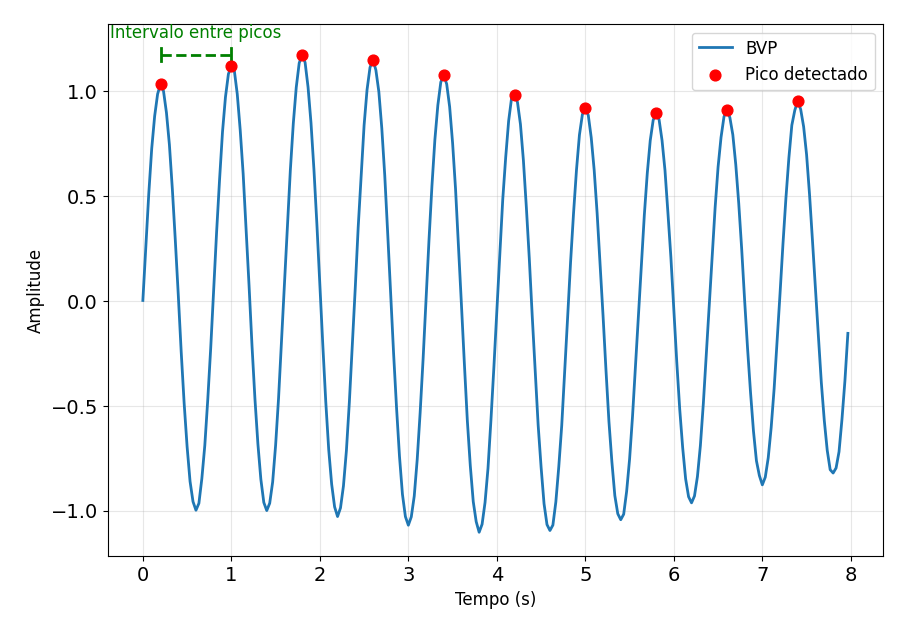
\includegraphics[width=\linewidth]{imagens/dominio_tempo.png}
\caption{}
\label{fig:fc_tempo}
\end{subfigure}
\hfill
\begin{subfigure}{0.45\textwidth}
\centering
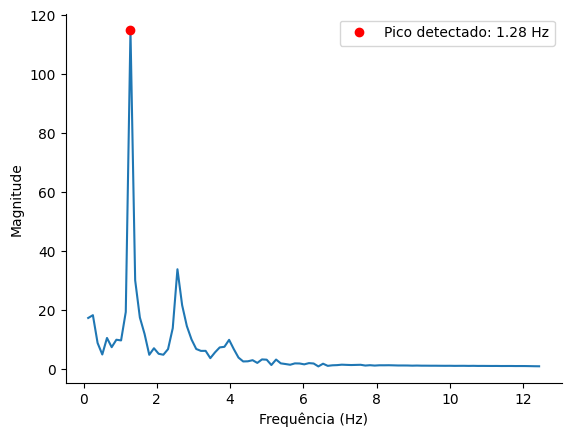
\includegraphics[width=\linewidth]{imagens/dominio_freq.png}
\caption{}
\label{fig:fc_freq}
\end{subfigure}

\caption{Representação de técnicas de estimativa da frequência cardíaca no domínio do tempo (a) e no domínio da frequência (b). No domínio do tempo, os picos do sinal de rPPG são detectados e, a partir da média de intervalo entre picos, a frequência cardíaca é estimada. No domínio da frequência, a estimativa de FC é realizada por meio da identificação do primeiro pico mais proeminente no espectro da série temporal do sinal de rPPG, correspondente à frequência fundamental.}
Fonte: autoria própria
\label{fig:det_freq_card}
\end{figure}

% Citar métodos supervisionados para extração da frequência cardíaca \cite{vspetlik2018visual}

\subsection{Variabilidade da frequência cardíaca}

A variabilidade da frequência cardíaca (HRV) refere-se à variação do intervalo de tempo entre batimentos cardíacos consecutivos e permite a avaliação da saúde do sistema cardíaco, especialmente do funcionamento do sistema nervoso autônomo responsável por sua regulação \cite{acharya2006heart}. Esse parâmetro é comumente calculado com base no eletrocardiograma, no entanto pode ser estimado de maneira consistente pela variabilidade da frequência de pulso baseada na onda de PPG para indivíduos em repouso \cite{schafer2013accurate}. Para isso, analisa-se a variação dos intervalos entre picos ao longo do tempo da onda de pulso de volume sanguíneo. 

No contexto da fotopletismografia remota, é demonstrado que a estimativa da frequência cardíaca pode ser obtida com acurácia satisfatória por meio da identificação da frequência predominante do espectro do sinal obtido por câmera. Todavia, a identificação dos intervalos entre batimentos ainda apresenta-se como um desafio. Isso ocorre devido sobretudo à necessidade da detecção precisa de picos do sinal, a qual requer uma relação sinal-ruído adequada que normalmente não é obtida pela medição remota, e devido à necessidade de uma frequência de amostragem mínima para a obtenção de valores de HRV confiáveis, especificamente de 100 Hz no caso da obtenção a partir do eletrocardiograma \cite{malik1996heart}. No caso da obtenção a partir do sinal de PPG, é possível verificar que a obtenção de medidas de HRV tanto no domínio do tempo quanto no domínio da frequência a partir do sinal de fotopletismografia amostrado a 1000 Hz pode ser comparável a medidas obtidas a partir do sinal amostrado a 50 Hz \cite{pelaez2021impact}, valor que, no entanto, não é comumente atingido por câmeras convencionais.

Apesar disso, é possível demonstrar que a interpolação do sinal de rPPG obtido com taxas de quadros menores do que a necessária gera resultados de estimativa de variabilidade da frequência cardíaca próximos aos obtidos com a taxa mínima e com boa correlação quando comparados aos obtidos por sensores de contato \cite{sun2013noncontact}. Ademais, estratégias de otimização da detecção dos picos da onda de BVP medida remotamente contribuem para a obtenção de valores do intervalo entre picos com boa correlação em relação aos valores de referência \cite{maki2019inter, li2020video}. Analogamente, soluções de aprendizado profundo focadas na redução do ruído dos sinais de crominância capturados por câmera para geração de formas de onda de BVP realistas permitem a otimização da acurácia da estimativa do intervalo entre pulsos e, consequentemente dos parâmetros relacionados à variabilidade de frequência cardíaca  \cite{Song2021pulsegan, yang2023cbppggan}. 

\subsection{Frequência respiratória}

A onda de fotopletismografia reflete a pulsação cardiogênica ao representar as variações temporais no volume sanguíneo periférico, decorrentes da propagação da onda de pulso ao longo do ciclo cardíaco. No entanto, o sinal fotopletismográfico também é influenciado pelo sistema respiratório, de forma que a onda de pulso de volume sanguíneo característica da fotopletismografia também é modulada por três principais fatores relacionados à respiração, conforme exibido na \autoref{fig:resp-mods}. Primeiramente, há uma modulação da linha de base do sinal, induzida pelo retorno venoso causado pelas mudanças na pressão intratorácica que acontecem durante a inspiração e a expiração. Além disso, essas mudanças de pressão resultam em variações do volume de sangue expelido pelo ventrículo esquerdo, o que gera uma modulação de amplitude da onda. Por fim, há uma modulação da frequência do sinal de PPG gerada pela variação da frequência cardíaca ao longo do ciclo respiratório, em que há a redução do período cardíaco durante a inspiração e um aumento ao longo da expiração devido à atuação do sistema nervoso autônomo, fenômeno denominado arritmia sinusal respiratória. Assim, os efeitos desses fatores podem ser identificados, o que faz com que seja possível extrair informações da respiração pela onda característica de PPG com o uso de algoritmos os quais também podem ser aplicados ao sinal obtido remotamente \cite{luguern2020assessment}. 

\begin{figure}[h!]
    \centering
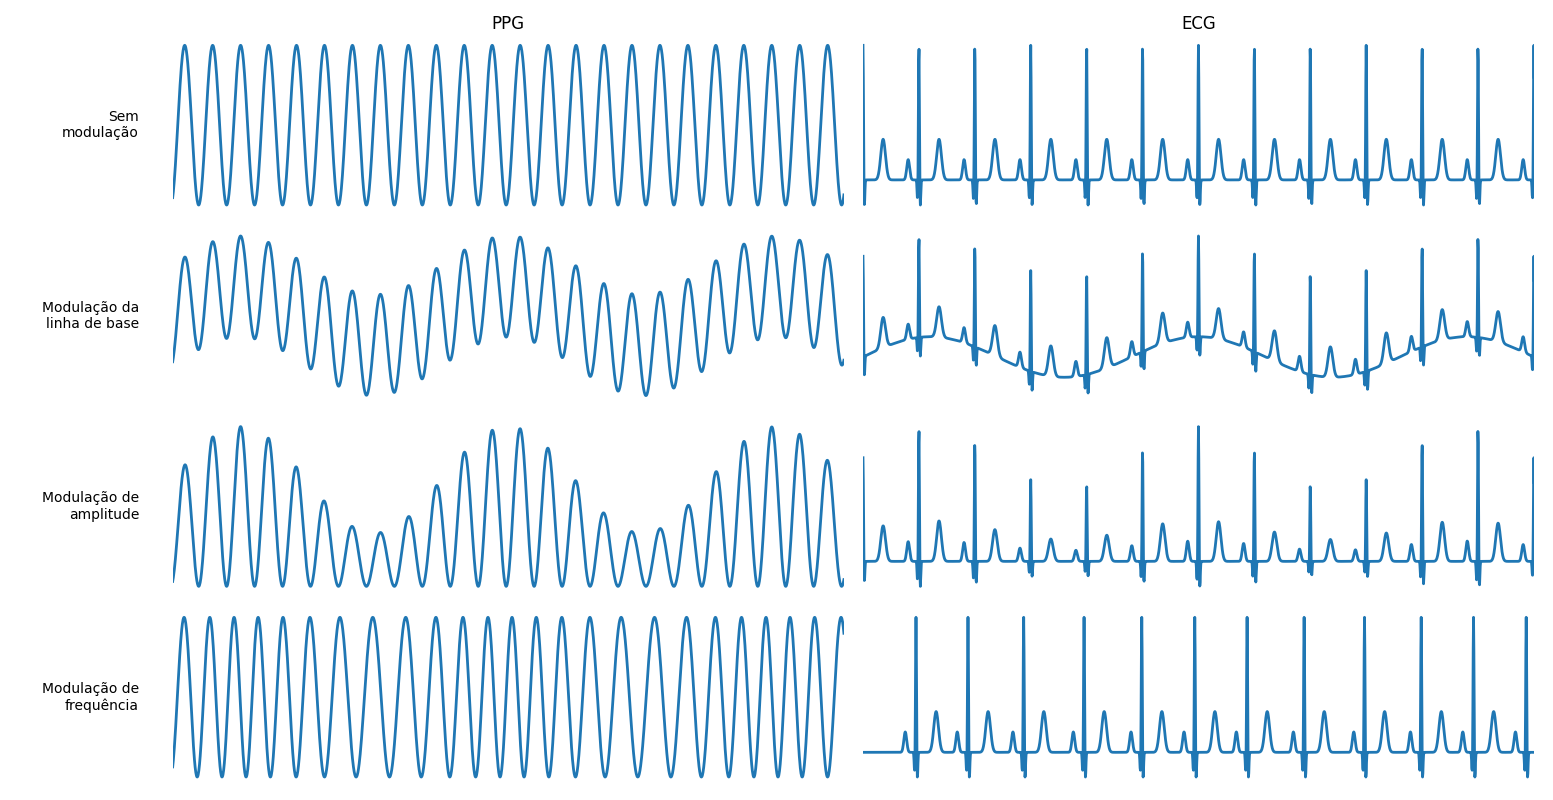
\includegraphics[width=\linewidth]{imagens/resp_mods.png}
    \caption{Exemplos das modulações respiratórias observadas em sinais de fotopletismografia (PPG) e eletrocardiografia (ECG). A primeira linha apresenta os sinais sem influência respiratória. As linhas subsequentes ilustram, respectivamente, a modulação da linha de base, caracterizada pelo deslocamento periódico do nível médio do sinal; a modulação de amplitude, associada a variações na amplitude dos picos; e a modulação de frequência, relacionada às alterações cíclicas no espaçamento entre picos consecutivos do sinal.}
    Fonte: Adaptado de \citeonline{charlton2016assessment}
    \label{fig:resp-mods}
\end{figure}

No contexto do monitoramento por câmera, duas das principais abordagens envolvem detectar as modulações induzidas pelo ciclo respiratório no sinal de rPPG ou detectar as variações induzidas pelo movimento causado pela respiração \cite{wei2017non, schrumpf2019exploiting}, sendo que a primeira atinge melhor acurácia e apresenta maior confiabilidade \cite{boccignone2023evaluation}. De fato, é possível demonstrar que essas modulações podem ser identificadas pela análise das variabilidades da largura, da frequência e da amplitude de pulso \cite{iozzia2017respiratory}. Mais recentemente, soluções de aprendizado profundo permitem a obtenção de sinais cardíaco e respiratório a partir de modelos multi-tarefas \cite{lee2022multitask, liu2020multi}. 

\subsection{Saturação periférica de oxigênio (SpO2)}

A saturação periférica de oxigênio (SpO2) corresponde à razão entre as concentrações da hemoglobina oxigenada e da hemoglobina total presente no sangue, sendo que há diferenças significativas entre a absorção de luz pela oxihemoglobina e pela desoxihemoblobina ao longo dos diversos comprimentos de onda, de forma proporcional às respectivas concentrações. Assim, a fotopletismografia permite a identificação desse parâmetro por meio da análise da razão entre as amplitudes da componente AC do sinal sob iluminações referentes ao vermelho e ao infravermelho próximo, bem como da componente DC correspondente. A escolha desses comprimentos de onda se dá devido à diferença de absorção das duas substâncias, o que faz com a comparação seja sensível a mudanças na oxigenação \cite{allen2007photoplethysmography}. 

Diferente da medição por contato, a estimativa da SpO2 a partir do sinal obtido remotamente deve levar em consideração a região do espectro luminoso capaz de ser capturada pelo sensor óptico da câmera sob iluminação ambiente. Nesse sentido, as soluções nesse contexto utilizam a comparação entre o vermelho e o verde, considerando as diferenças de absorção pela oxihemoglobina e pela desoxihemoglobina nesses comprimentos de onda \cite{kong2013non}, apesar de a profundidade atingida no tecido cutâneo ser menor na faixa do verde, quando comparada ao infravermelho próximo e ao vermelho \cite{mocco2021pulse}. Outras implementações demonstram, ainda, que a utilização dos sinais dos canais azul e vermelho gera resultados comparáveis aos obtidos por um oxímetro de pulso \cite{casalino2020mhealth, gs2024remote, guazzi2015non}.

\subsection{Pressão arterial}

A pressão sanguínea refere-se à força que o sangue exerce contra as paredes dos vasos sanguíneos enquanto circula pelo sistema cardiovascular. Esse parâmetro é frequentemente medido de forma invasiva por cateterismo ou de forma não invasiva por ausculta ou método oscilométrico com a utilização de manguitos pressurizados. No entanto, há soluções que estimam esse sinal a partir do tempo de trânsito de onda de pulso (\textit{Pulse Transit Time} - PTT), o qual corresponde ao tempo que a onda de pressão leva para percorrer duas regiões diferentes do sistema arterial. No contexto da fotopletismografia, a medição do PTT pode ser realizada por meio da comparação dos sinais de dois oxímetros medidos em locais distintos \cite{mukkamala2015toward}. 

No cenário do monitoramento remoto, por sua vez, o tempo de trânsito de onda de pulso  pode ser obtido a partir de duas medições remotas realizadas em locais diferentes, como na região do pé e da mão \cite{murakami2015non} ou na região do rosto em comparação com a palma da mão \cite{fan2020robust}. Por fim, a partir do PTT, a pressão sanguínea é estimada por meio de estratégias de calibração. Outras soluções aproximam esse parâmetro pelo tempo de chegada de pulso (\textit{Pulse Arrival Time} - PAT) estimado como o tempo entre o pico R do ECG e o pé do sinal de rPPG extraído do rosto \cite{secerbegovic2016blood}.

Soluções mais recentes, por outro lado, permitem a estimativa da pressão sanguínea remotamente com base na análise unicamente da região do rosto. Para isso, são implementadas estratégias de aprendizado de máquina, por exemplo, para relacionar esse parâmetro com a distribuição espacial e temporal do sinal de pulso facial utilizando modelos de redes neurais convolucionais \cite{iuchi2022blood} ou uma combinação desse tipo de modelo para extrair características espaciais com redes neurais recorrentes para análise temporal \cite{hamoud2023neural}. É possível, ainda, relacionar a pressão sanguínea com o sinal de rPPG e outros indicadores fisiológicos, como a frequência cardíaca e o tempo de trânsito da onda de pulso, com o uso de redes neurais profundas \cite{wu2022facial}.


% \subsection{Perfusão sanguínea periférica}

\newpage\chapter{Materiais e métodos}

Este projeto adota um delineamento observacional, prospectivo e analítico, com o objetivo de validar algoritmos de rPPG para extração de sinais fisiológicos em pacientes críticos internados na UTI do Hospital Universitário da Universidade de São Paulo. O estudo foi aprovado pelo Comitê de Ética em Pesquisa da instituição sob o número Certificado de Apresentação de Apreciação Ética (CAAE) 86650625.3.0000.0076. Todos os dados são coletados com permissão explícita dos indivíduos envolvidos ou de seus representantes. 

\section{Aquisição de dados}

A aquisição de dados é realizada por meio da gravação de vídeos da face de pacientes internados na UTI realizada com uma câmera industrial sob condições de iluminação ambiente do leito e sem imposição de nenhuma restrição ao indivíduo monitorado. Cada gravação tem duração aproximada de dois minutos e a câmera é posicionada ao pé da cama hospitalar, conforme demonstra a Figura \ref{fig:setupcoleta}, caso o paciente esteja deitado, ou a uma distância fixa próxima de 180 centímetros, caso o paciente esteja sentado na poltrona também disponível no local de internação. Ademais, são coletados dados sobre a iluminação medida na região próxima ao rosto, com o uso de um luxímetro digital de modelo Fluke 941 e é realizada a medição do fototipo de acordo com a escala Fitzpatrick com um Analisador de Fototipo de Pele Digital da \textit{Skinup Beauty Devices} posicionado na testa. Simultaneamente, são extraídos dados fisiológicos de referência do sinal do eletrocardiograma com taxa de amostragem de 250 Hz, da frequência respiratória com taxa de amostragem de 125 Hz e da onda de fotopletismografia obtida por meio de um oxímetro de pulso com taxa de amostragem de 62,5 Hz. Todos os sinais fisiológicos são adquiridos diretamente dos monitores multiparâmetros de modelo BSM-3000 Series da Nihon Kohden já instalados à beira-leito, utilizando um sistema de coleta previamente implementado para comunicação com os dispositivos.

\begin{figure}[h]
    \centering
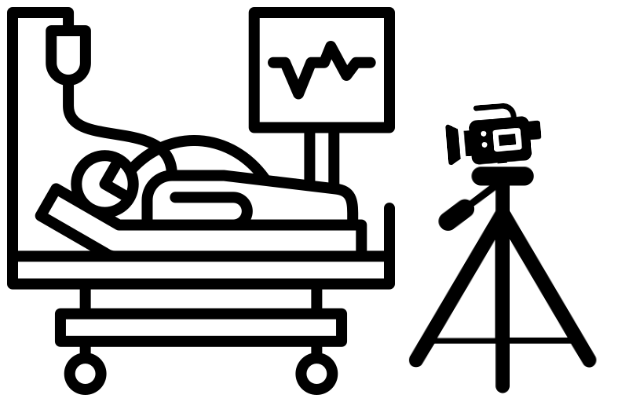
\includegraphics[width=0.5\linewidth]{imagens/setup_coleta.png}
    \caption{Esquemático do ambiente de coleta de dados} 
    Fonte: autoria própria
    \label{fig:setupcoleta}
\end{figure}

A aquisição de dados foi estruturada em três procedimentos diferentes, sendo eles:

\begin{enumerate}
    \item \textbf{Coleta preliminar}

    Foi realizada uma coleta preliminar de dados de três pacientes internados na UTI, com uma câmera do modelo VCXG.2-57C da Baumer configurada com taxa de 25 quadros por segundo, formato de pixel BR8. Para cada paciente, o tempo de exposição, ganho, foco e abertura do sensor foram definidos de forma a garantir a máxima visualização com o mínimo de sombras e sem saturação de pixels. A resolução, por sua vez, foi definida de forma a enquadrar o rosto e parte do tórax e os vídeos são capturados em formato AVI. Além disso, a distância entre cada indivíduo e a câmera variou de acordo com a disposição do paciente dentro do ambiente de internação, sendo que esse valor variou entre 170 e 190 centímetros, já que dois dos pacientes estavam deitados na cama reclinada e um dos pacientes estava sentado em uma poltrona ao lado da cama.  

    \item \textbf{Coleta de validação}

    Em um segundo momento, foi realizada a coleta de três vídeos em formato AVI de 2 minutos e 5 segundos de duração de um indivíduo saudável não hospitalizado com uma câmera do modelo VCXU.2-57C com 50 quadros por segundo, com uma resolução fixa de 1056x1076 e tempo de exposição fixo em 19500 milissegundos. O ganho, foco e abertura do sensor foram definidos de forma a garantir a máxima visualização com o mínimo de sombras e sem saturação de pixels. Além disso, a distância entre o indivíduo e a câmera foi definida como 140 centímetros. Nesse caso, foi adquirido o sinal de eletrocardiograma com um equipamento de eletromiografia e registro de potenciais evocados do modelo MEB-2300K da Nihon Kohden com frequência de amostragem de 1000 Hz e eletrodos posicionados no dorso das mãos e nos tornozelos para a medição da derivação DII. No início de cada gravação, foi gerado um ruído em um eletrodo de ECG visível no enquadramento para sincronização posterior entre os quadros capturados e o sinal de referência, conforme será elaborado adiante. Esse procedimento foi executado com o intuito de validar a aplicação dos algoritmos considerados, os quais serão expostos em diante, em um indivíduo saudável.

    \item \textbf{Coleta definitiva}

    Para a coleta definitiva, serão adquiridos vídeos de 2 minutos e 5 segundos de duração de ao menos 10 pacientes com a câmera de modelo VCXU.2-57C com 50 quadros por segundo, sob os mesmos procedimentos de ajuste do sensor óptico que os adotados na coleta de validação. Nesse caso, a distância entre a câmera e o paciente é condicionada pela disposição da instalação e pelo posicionamento do indivíduo dentro dela. Ademais, os dados de referência serão coletados dos monitores multiparâmetros, da mesma maneira descrita para a coleta preliminar.

\end{enumerate}

A diferença da câmera em cada procedimento se dá devido à disponibilidade, dado que a coleta preliminar foi realizada com uma câmera provisória disponibilizada pela empresa fabricante, enquanto as outras coletas dependem da aquisição definitiva do segundo modelo. Ademais, a escolha da utilização de uma câmera industrial é baseada sobretudo no objetivo de garantir a aquisição de dados sem compressão, já que esse é um fator que deteriora significativamente a relação sinal-ruído, conforme discutido na \autoref{sec:influencing-factors}. Além disso, a obtenção de imagens de boa qualidade em um sistema cujos parâmetros do sensor óptico podem ser configurados de forma acessível garante a robustez na análise dos algoritmos. 

\subsection{Sincronização de dados}

A aquisição dos dados de vídeo é realizada com a duração de aproximadamente 2 minutos, ao passo que os dados de referência, em todos os procedimentos de coleta, são gravados em um intervalo de tempo maior que o do vídeo e que abrange o momento de sua gravação. Assim, é necessária a sincronização desses sinais para o posterior processamento e análise. Isso é realizado com base na comparação entre o horário de aquisição dos vídeos e os registros temporais referentes aos sinais fisiológicos. Como esses horário não são necessariamente coincidentes, apesar de sempre serem próximos, são necessárias etapas específicas a cada procedimento de coleta de dados. 

\begin{itemize}
    \item \textbf{Coleta preliminar}

    O único protocolo de sincronização de dados nesse procedimento de coleta foi o registro dos horários de início e fim da gravação do vídeo e do horário apresentado no monitor multiparâmetros no instante do início da gravação. Desse modo, como os dados de referência são capturados de forma contínua, a sincronização dos dados de uma captura de vídeo específica baseia-se na obtenção do intervalo de tempo dentro dos registros temporais dos sinais de referência na qual foi realizada essa captura. Para isso, é aplicada uma análise de correlação entre os valores de frequência cardíaca estimados a partir dos sinais obtidos remotamente e os valores de referência extraídos do ECG em um intervalo suficientemente grande. 
    
    Dessa maneira, assume-se que a diferença entre os relógios do sistema de armazenamento dos dados dos monitores e do computador responsável por registrar os vídeos não excede três minutos. Dessa forma, define-se uma janela temporal de oito minutos que engloba o horário indicado pelo monitor no momento da aquisição. A partir dessa janela, são extraídos os dados brutos do ECG e a frequência cardíaca é estimada utilizando a biblioteca HeartPy \cite{heartpy}, com janelas deslizantes de 15 segundos e passo de um segundo. Em paralelo, os sinais de BVP são obtidos a partir dos vídeos por meio de 7 métodos não supervisionados de rPPG, os quais serão expostos adiante, sendo que os vídeos foram subdivididos em janelas de 15 segundos. Para cada janela, a frequência cardíaca é estimada no domínio da frequência por meio da FFT, considerando o pico espectral do sinal previamente filtrado na faixa de 0,6 a 3,3 Hz. Por fim, para cada método de rPPG, as séries temporais de frequência cardíaca obtidas remotamente e as séries obtidas a partir do ECG são alinhadas por meio de uma análise de correlação cruzada baseada no índice de correçação de Pearson, na qual a série derivada da rPPG é transladada temporalmente em relação à série de referência do ECG, com passo de um segundo, conforme é explicitado na Figura \ref{fig:sinc-L9} do \autoref{cap:results}. Desse modo, o intervalo de dois minutos, que é o tempo de duração de cada vídeo, que apresenta o maior coeficiente de correlação médio é selecionado para a extração final dos dados de referência.

    \item \textbf{Coleta de validação}

    Nessa coleta, em cada gravação, foi gerado um ruído em um dos eletrodos de eletrocardiograma do indivíduo monitorado de forma visível no enquadramento da imagem da câmera. Assim, o primeiro quadro do vídeo em que é identificada a interferência no eletrodo é utilizado de forma que os quadros anteriores são desconsiderados. Além disso, o vídeo é cortado de modo que são consideradas as imagens capturadas 5 segundos após esse quadro para a extração do sinal sem a interferência desse artefato. Ademais, o ruído gerado, causado por um impacto no eletrodo, gera um pico distinguível na forma de onda do sinal de ECG, de forma que o intervalo considerado para o sinal de referência possui início no instante 5 segundos após o momento respectivo a esse pico e tem duração igual à do vídeo correspondente já editado. 

    \item \textbf{Coleta definitiva}

    Nessa coleta, serão realizados os mesmos procedimentos de sincronização de dados adotados na coleta de validação.
    
\end{itemize}

\section{Processamento de dados de vídeo}

Os dados de vídeo são processados com o uso do conjunto de ferramentas de código aberto denominado rPPG-Toolbox \cite{liu2022rppg}, o qual disponibiliza implementações dos principais métodos não supervisionados de extração de sinais por fotopletismografia remota. Além disso, esse recurso inclui modelos supervisionados para treinamento e teste em bases de dados de acesso livre, além de permitir a inclusão de modelos e bases customizados. Com isso, propõe-se a validação dos algoritmos mostrados na \autoref{tab:metodos_rppg} nos dados coletados dos pacientes de UTI, por meio da inserção de um dataset customizado e da adaptação do conjunto de ferramentas citado.

\begin{table}[ht]
\centering
\caption{Métodos a serem validados nos dados coletados de pacientes de UTI}
\label{tab:metodos_rppg}
\begin{tabular}{|c|l|p{5cm}|}
\hline
\textbf{Tipo} & \textbf{Método} & \textbf{Estratégia} \\ \hline

\multirow{12}{*}{Não supervisionado}
& GREEN \cite{verkruysse2008remote} & Análise do canal verde\\ \cline{2-3}
& ICA \cite{poh2010advancements} & Separação cega de sinais \\ \cline{2-3}
& CHROM \cite{de2013robust} & Modelo baseado em crominância \\ \cline{2-3}
& PBV \cite{de2014improved} & Modelo do vetor de pulso \\ \cline{2-3}
& POS \cite{wang2016algorithmic} & Projeção no subespaço ortogonal ao tom de pele\\ \cline{2-3}
& LGI \cite{pilz2018local} & Modelagem de variações espaciais para robustez a movimento \\ \cline{2-3}
& OMIT \cite{casado2023face2ppg} & Modelagem baseada em decomposição de matrizes \\ \hline

\multirow{7}{*}{Supervisionado}
& DeepPhys \cite{chen2018deepphys} & CNN 2D com mecanismo de atenção \\ \cline{2-3}
& TSCAN \cite{liu2020multi} & CNN 2D com módulos de deslocamento temporal \\ \cline{2-3}
& PhysNet \cite{yu2019physnet} & CNN 3D \\ \cline{2-3}
& PhysFormer \cite{yu2022physformer} & Transformer Visual \\ \cline{2-3}
& EfficientPhys \cite{liu2023efficientphys} & Swin Transformer\\ \hline

\end{tabular}
\end{table}

Para isso, em cada vídeo de entrada, é realizada a detecção da face utilizando a ferramenta YOLO5Face \cite{qi2022yolo5face} a cada 25 quadros, sendo que a região de interesse selecionada é a região retangular retornada por essa ferramenta. Em seguida, os quadros recortados nessa região são utilizados como entrada para os algoritmos de rPPG. No caso especificamente dos algoritmos não supervisionados, é realizada, ainda, a média espacial dos pixels de cada quadro para o processamento das variações das intensidades dos canais de cor. Em relação à validação dos métodos baseados em aprendizado profundo, serão considerados os modelos treinados no dataset denominado PURE \cite{stricker2014pure} e no dataset referido como UBFC-rPPG \cite{bobbia2019unsupervised}.

A partir da onda de pulso resultante dos algoritmos considerados, a frequência cardíaca é estimada por análise em frequência utilizando a FFT em janelas subsequentes de 15 segundos, sendo que o pico do espectro de potência do sinal filtrado por um filtro passa-banda entre as bandas de 0,6 e 3,3 Hz é considerado como a frequência cardíaca. Ademais, a frequência respiratória pode ser estimada por três métodos de análise das modulações do sinal de rPPG causadas pela respiração, sendo eles a análise da modulação de linha de base (BW), a análise da modulação de amplitude (AM) e a análise da modulação de frequência (FM). Para isso, o sinal inicial extraído com um dos algoritmos de rPPG definidos é filtrado por um filtro passa-altas na banda referente a 4 respirações por minuto. Cada um dos métodos é aplicado em cada ponto do ciclo da onda de pulso extraída remotamente para obter a respectiva sequência discreta de amostras correspondente ao tipo de modulação em questão. 

A análise da modulação de linha de base baseia-se na média entre as amplitudes de um ponto de vale e do pico subsequente, conforme a equação:

\begin{equation}
    \label{eq:B}
    BW(n) = \frac{A_{vale}(n) + A_{pico}(n)}{2}
\end{equation}

em que \(A_{vale}(n)\) é a amplitude do vale de um ponto \(n\) da onda de rPPG e \(A_{pico}(n)\) é a amplitude do pico subsequente a esse ponto. A implementação desse cálculo em todos os ciclos do sinal permite extrair a sequência discreta de amostras \(BW\) da linha de base do sinal de rPPG, conforme mostra a \autoref{fig:bw}.

\begin{figure}[h!]
    \centering
    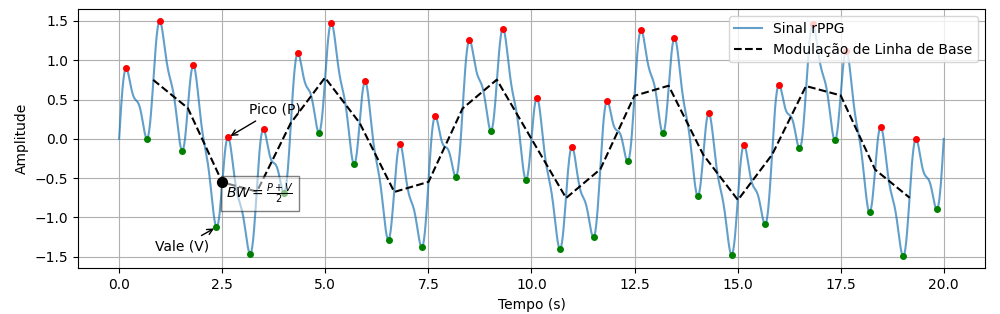
\includegraphics[width=0.9\linewidth]{imagens/bw.png}
    \caption{Extração da modulação de linha de base no sinal de rPPG causada pela respiração}
    Fonte: autoria própria
    \label{fig:bw}
\end{figure}

A análise da modulação de amplitude do sinal de rPPG causada pela respiração é baseada na diferença entre as amplitudes de um ponto de vale e do pico subsequente, conforme a equação:

\begin{equation}
    \label{eq:am}
    AM(n) = A_{pico}(n) - A_{vale}(n)
\end{equation}

em que \(AM\) é a sequência discreta de amostras da modulação de amplitude do sinal de rPPG, como exemplifica a \autoref{fig:am}.

\begin{figure}[h!]
    \centering
    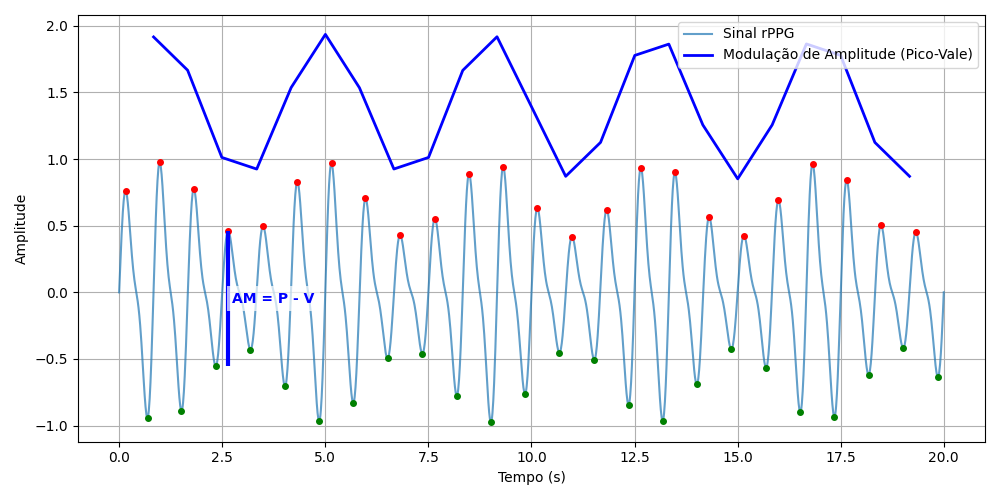
\includegraphics[width=0.9\linewidth]{imagens/am.png}
    \caption{Extração da modulação de amplitude do sinal de rPPG causada pela respiração}
    Fonte: autoria própria
    \label{fig:am}
\end{figure}

A análise da modulação de frequência no sinal de rPPG causada pelos fenômenos respiratórios, por sua vez, é realizada  considerando o intervalo entre picos consecutivos, de acordo com a equação:

\begin{equation}
    \label{eq:fm}
    FM(n) = t(n) - t(n-1)
\end{equation}

em que \(t(n)\) é o instante referente ao pico \(n\) e \(t(n-1)\) é o instante referente ao pico anterior. A implementação desse cálculo em todos os ciclos do sinal permite extrair a sequência discreta de amostras \(FM\) dos intervalos entre picos do sinal de rPPG, conforme mostra a \autoref{fig:fm}.

\begin{figure}[h!]
    \centering
    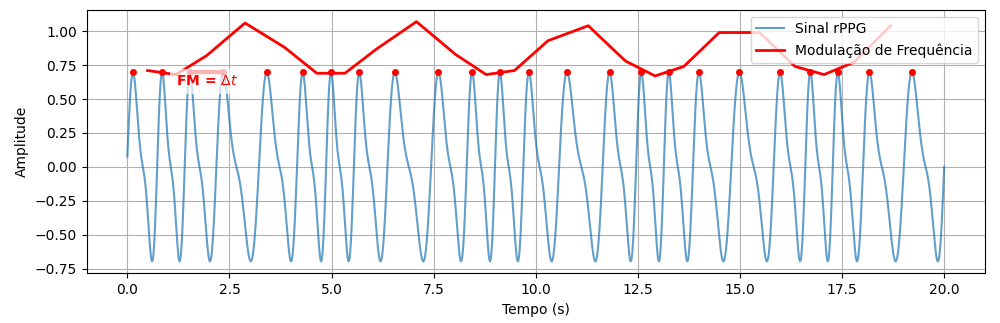
\includegraphics[width=0.9\linewidth]{imagens/fm.png}
    \caption{Extração da modulação de frequência do sinal de rPPG causada pela respiração}
    Fonte: autoria própria
    \label{fig:fm}
\end{figure}

Assim, as sequências discretas referentes às modulações de amplitude e de linha de base são re-amostradas em uma grade temporal uniforme de 4 Hz por meio de interpolação linear. Já a sequência referente à modulação de frequência é re-amostrada em uma grade temporal uniforme de 4 Hz por meio do algoritmo de Berger \cite{berger1986efficient}, uma vez que é derivada de intervalos entre picos do sinal de pulso obtido remotamente e não representa uma amostragem pontual do sinal no tempo. A partir disso, a frequência respiratória é estimada a partir de cada uma das sequências interpoladas por meio de análise espectral, de forma que a frequência com maior energia no espectro de potência obtido por FFT dentro das bandas esperadas nesse contexto, de 4 a 65 respirações por minuto, é considerada como o valor de frequência respiratória obtido pelo método correspondente. Esse processo é realizado em janelas subsequentes de 30 segundos do sinal de rPPG original. Em seguida, a fim de reduzir interferências de artefatos de ruído, é realizada uma estratégia de fusão das estimativas de frequência respiratória realizadas pelos 3 métodos, de modo que a estimativa final é uma média desses 3 valores. No entanto, de maneira a garantir a robustez dessa estratégia, esse valor só é considerado confiável caso o desvio padrão entre as estimativas seja menor que 4 respirações por minuto \cite{charlton2016assessment, luguern2020assessment}.

\section{Processamento dos dados de referência}

Paralelamente, para a construção da base de dados proposta, são utilizados os dados de referência coletados dos monitores multiparâmetros e devidamente sincronizados com os vídeos. Para tanto, é extraído o sinal do eletrocardiograma considerado como padrão-ouro para a obtenção da frequência cardíaca, sendo que esse parâmetro é calculado utilizando a biblioteca HeartPy \cite{heartpy}, com janelas de 15 segundos. A forma de onda fotopletismográfica, por sua vez, obtida com um oxímetro de pulso posicionado no dedo indicador, é utilizada para comparação com o sinal de pulso resultante dos algoritmos por meio de uma análise por correlação cruzada. Por fim, o sinal de impedância torácica captado pelos eletrodos de ECG também é extraído como referência para extração da frequência respiratória realizada utilizando a FFT em janelas subsequentes de 30 segundos. Exemplos desses sinais são apresentados na \autoref{fig:sinais-referencia}.

\begin{figure}[h!]
    \centering

    % Linha superior
    \begin{subfigure}{0.45\textwidth}
        \centering
        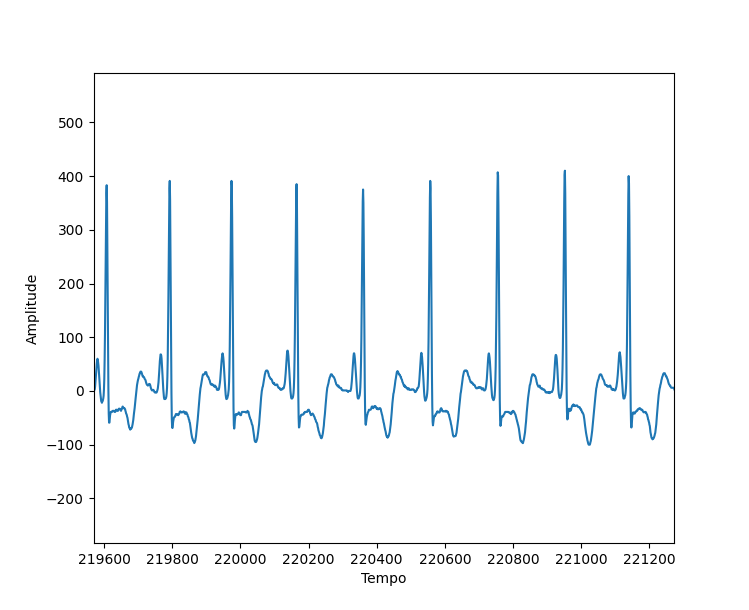
\includegraphics[width=\linewidth]{imagens/ecg_exemplo.png}
        \caption{ECG}
    \end{subfigure}
    \hfill
    \begin{subfigure}{0.45\textwidth}
        \centering
        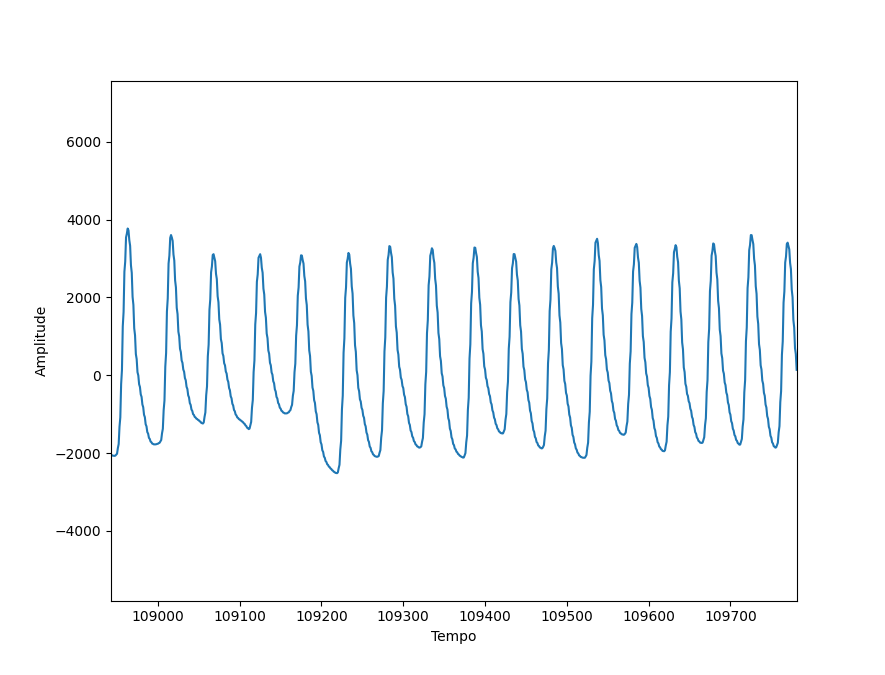
\includegraphics[width=\linewidth]{imagens/PPG_oximetro_exemplo.png}
        \caption{PPG}
    \end{subfigure}

    % Linha inferior
    \begin{subfigure}{0.6\textwidth}
        \centering
        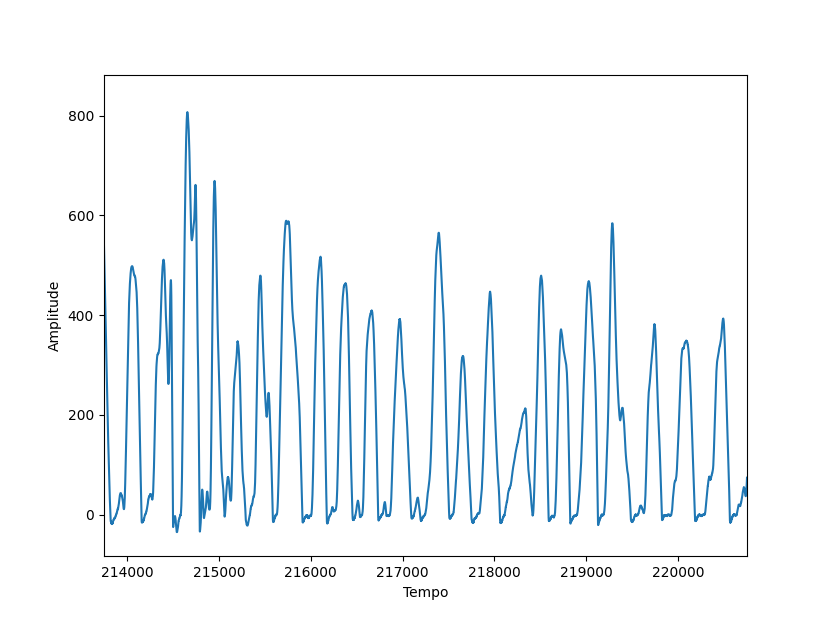
\includegraphics[width=\linewidth]{imagens/impedancia_toracica_exemplo.png}
        \caption{Impedância torácica}
    \end{subfigure}

    \caption{Exemplos de sinais de referência}
    \label{fig:sinais-referencia}
\end{figure}

\section{Métricas de avaliação}

Os parâmetros de frequência cardíaca e frequência respiratória são extraídos em janelas subsequentes do sinal de pulso obtido remotamente, assim como os valores de referência. Assim, são calculadas métricas de comparação entre as janelas coincidentes de cada sinal a fim de quantificar o desempenho de cada algoritmo na estimativa dos parâmetros considerados, de forma que os valores de frequência cardíaca estimados a partir do sinal de rPPG são comparados janela a janela com os valores estimados a partir do ECG. Os valores de frequência respiratória estimados a partir do sinal obtido remotamente, por sua vez, são comparados janela a janela com os valores estimados a partir do sinal de impedância torácica de referência. Nesse sentido, é definido a seguir o cálculo de cada métrica aplicada.

\textbf{Erro Absoluto Médio (MAE)} 
\begin{equation}
    MAE = \frac{1}{N} \sum_{n=1}^{N} \left| R_g - R_p \right|
\end{equation}

\textbf{Erro Quadrático Médio (RMSE)}
\begin{equation}
    RMSE = \sqrt{\frac{1}{N} \sum_{n=1}^{N} (R_g - R_p)^2}
\end{equation}

\textbf{Erro Percentual Absoluto Médio (MAPE)}
\begin{equation}
MAPE = \frac{1}{N} \sum_{n=1}^{N} \left| \frac{R_g - R_p}{R_g} \right|
\end{equation}

\textbf{Índice de Correlação de Pearson (\(\rho\))}
\begin{equation}
\rho = 
\frac{
\sum_{n=1}^{N} (R_{g,n} - \bar{R}_g)(R_{p,n} - \bar{R}_p)
}{
\sqrt{
\left( \sum_{n=1}^{N} (R_{g,n} - \bar{R}_g)^2 \right)
\left( \sum_{n=1}^{N} (R_{p,n} - \bar{R}_p)^2 \right)
}
}
\end{equation}

Em todas as equações, \(R_g\) é o valor de referência, \(R_p\) é o valor estimado por meio do sinal obtido remotamente, \(N\) é o número de amostras de janelas de 15 segundos considerado e \(\bar{R_g}\) e \(R_p\) são as médias desses valores ao longo das amostras. 

\textbf{Relação Sinal-Ruído (SNR)}
\begin{equation}
SNR = 10 \log_{10} \left(
\frac{
\sum_{f=45}^{150} \left( U_t(f) S(f) \right)^2
}{
\sum_{f=45}^{150} \left( (1 - U_t(f)) S(f) \right)^2
}
\right)
\end{equation}
Nesse caso, \(S\) é o espectro de frequência do sinal de rPPG, \(U_t(f)\) é uma função definida como 1 na frequência fundamental e no primeiro harmônico do sinal de referência e como 0 em todos os outros pontos.

\begin{figure}[h]
    \centering
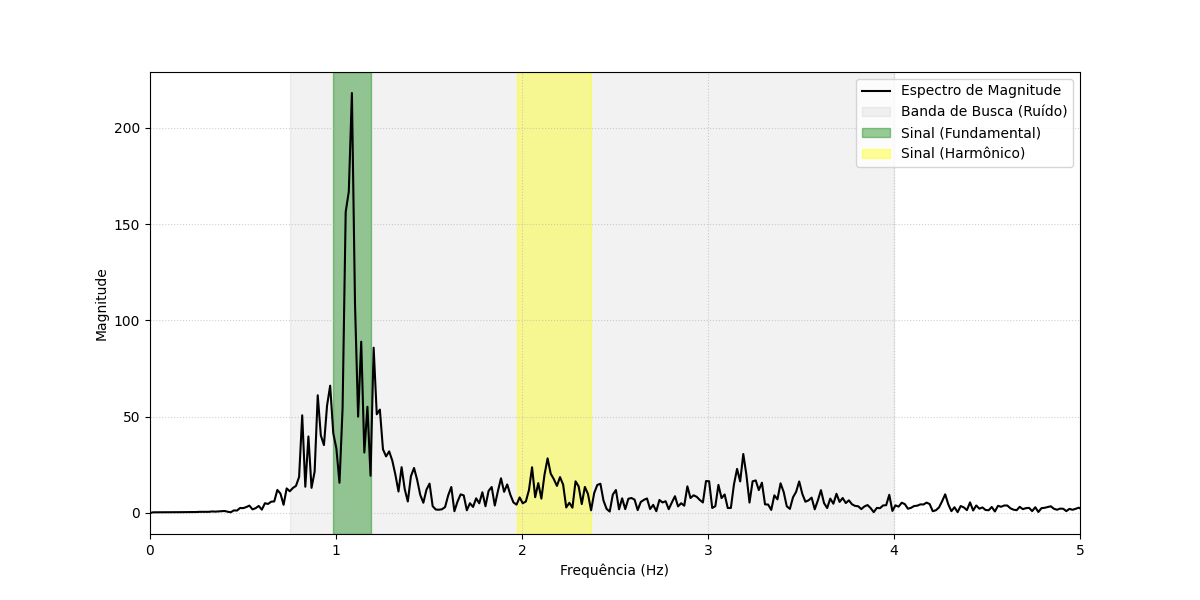
\includegraphics[width=1\linewidth]{imagens/snr_ex.png}
    \caption{Exemplo da definição da relação sinal-ruído}
    Fonte: autoria própria
    \label{fig:snr}
\end{figure}

Além disso, a fim de analisar as ondas de pulso de volume sanguíneo obtidas por cada método de rPPG, é realizada uma análise por correlação entre esse sinal e o sinal de fotopletismografia de referência, de modo que as duas ondas são sincronizadas por correlação cruzada e é calculado o índice de correlação de Pearson entre os sinais normalizados e sincronizados. Nesse caso, as amostras consideradas são os pontos do sinal de rPPG re-amostrado na frequência do sinal de referência. 


\newpage\chapter{Resultados preliminares}
\label{cap:results}

\section{Coleta preliminar}

Na coleta preliminar, foram adquiridos vídeos e os sinais correspondentes provenientes de monitores multiparamétricos de três pacientes admitidos na UTI. Em um dos casos, o oxímetro de pulso não estava conectado no momento da aquisição, impossibilitando a obtenção do sinal de fotopletismografia de referência. Entre os dois pacientes restantes, um encontrava-se sob suporte ventilatório mecânico e sedação, enquanto o outro estava em estado ativo e sem suporte ventilatório. A seguir, são expostos os resultados do processamento dos sinais obtidos. 

% L7 - paciente 1
% L9 - paciente 2
% L8 - paciente 3

\subsection{Sincronização de dados}

Para realizar a sincronização dos vídeos com os dados de referência, foi realizada uma análise de correlação baseada no índice de correlação de Pearson entre estimativas de frequência cardíaca realizadas a partir do eletrocardiograma e as estimativas realizadas a partir do sinal de rPPG extraído por cada um dos métodos não supervisionados citados na \autoref{tab:metodos_rppg}, conforme exemplifica a \autoref{fig:sinc-L9}. Com isso, foi obtido o gráfico de correlação média entre todos os métodos para cada paciente, como pode ser observado no exemplo da \autoref{fig:mean-corr-L9}. A partir do ponto de maior correlação em cada caso, foi obtido o intervalo a ser considerado para a extração dos dados de referência. 

\begin{figure}[h!]
    \centering
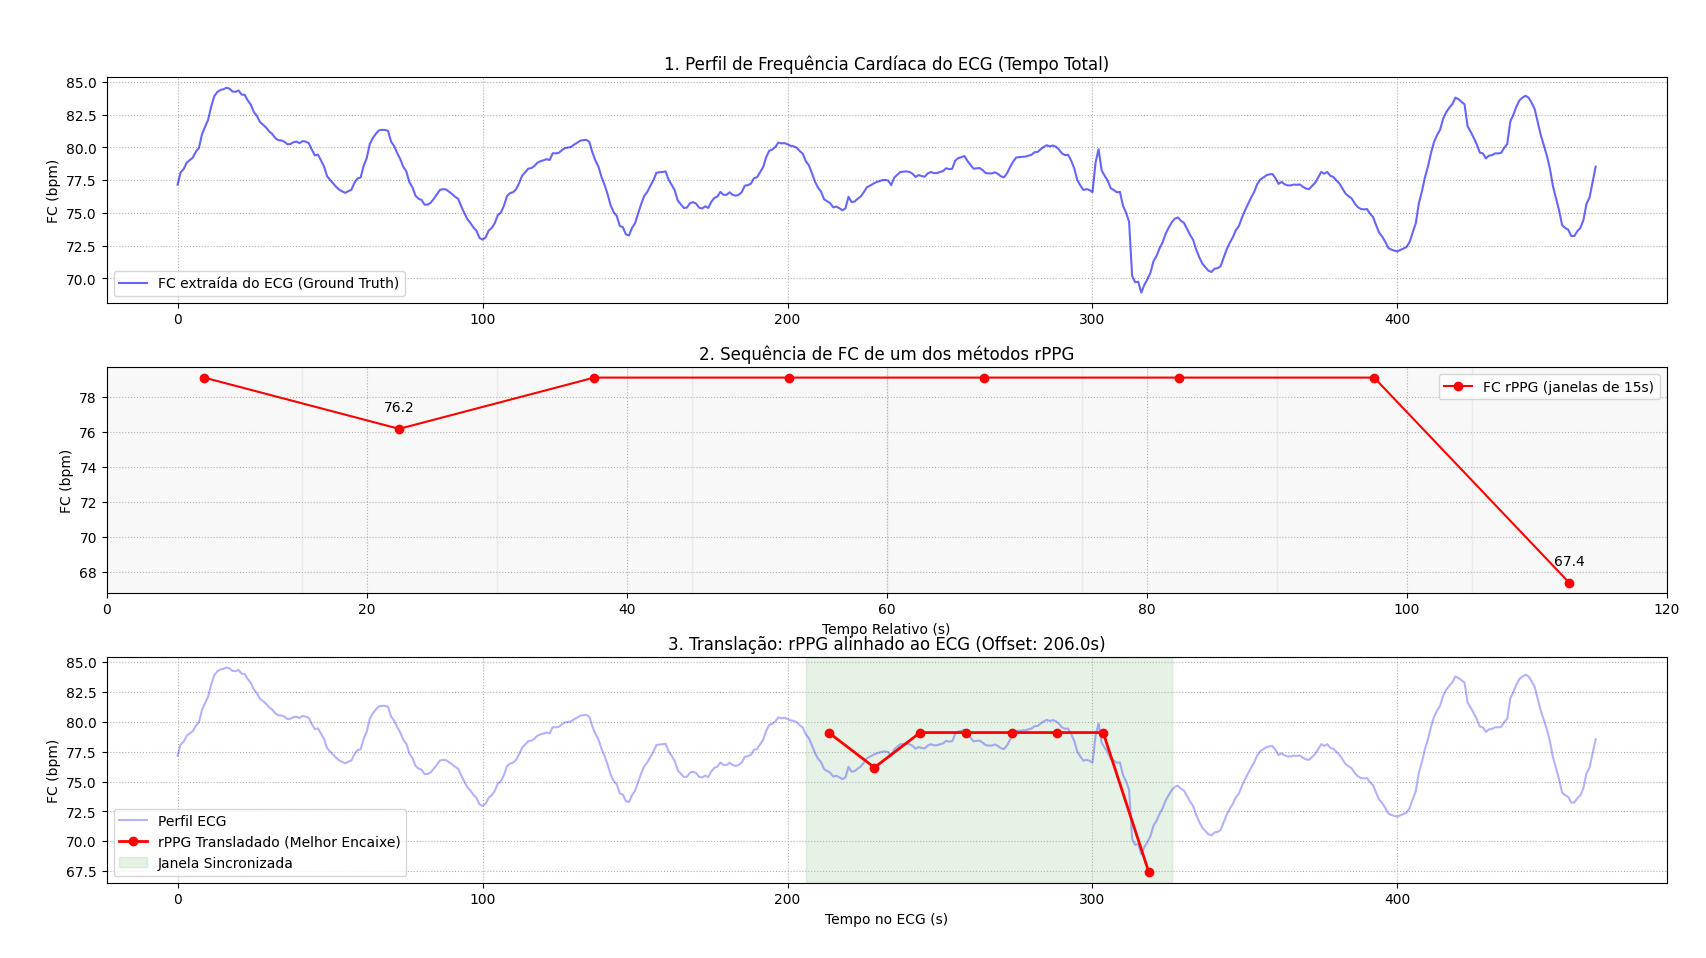
\includegraphics[width=1\linewidth]{imagens/hr_L9.png}
    \caption{Etapas de definição do intervalo considerado para os dados de referência do paciente 2}
    Fonte: autoria própria
    \label{fig:sinc-L9}
\end{figure}

\begin{figure}[h!]
    \centering
        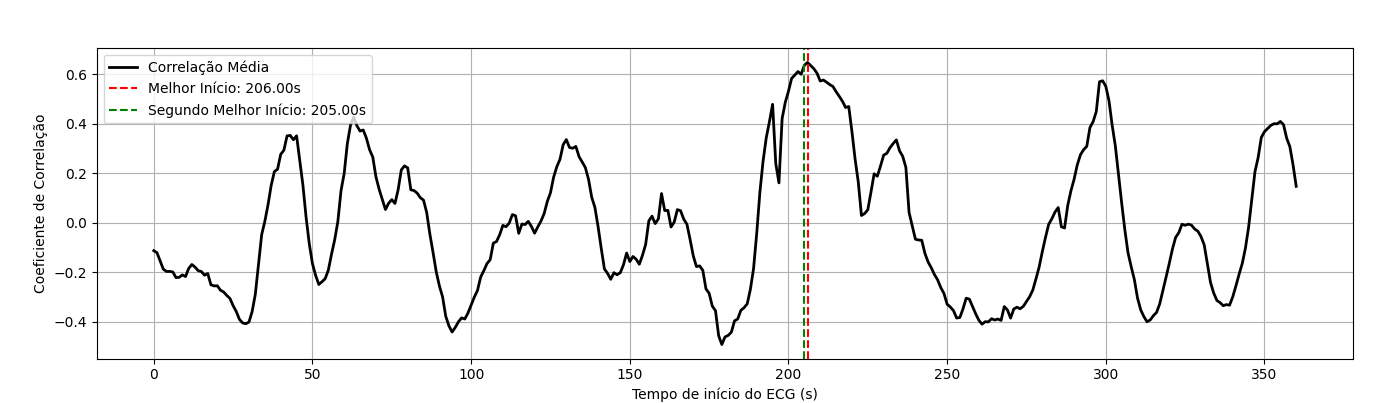
\includegraphics[width=\linewidth]{imagens/mean_corr_L9.png}
        \caption{Correlação média entre os valores de frequência cardíaca obtidos a partir do ECG de referência e os valores estimados pelos métodos de rPPG para o paciente 2}
        Fonte: autoria própria
        \label{fig:mean-corr-L9}
\end{figure}


Para o paciente 3, foi realizada a sincronização de forma similar à utilizada na coleta de validação, de forma que foi gerado um ruído no eletrocardiograma causado pela desconexão e reconexão de um dos eletrodos. Esse ruído insere um pico na forma de onda do ECG, conforme a \autoref{fig:ruido-ecg-L8}, sendo que considera-se o sinal no intervalo que se inicia 5 segundos após o momento respectivo a esse pico. Da mesma forma, o vídeo referente a esse paciente é cortado 5 segundos após o quadro em que se identifica a desconexão do eletrodo. 

\begin{figure}[h!]
    \centering
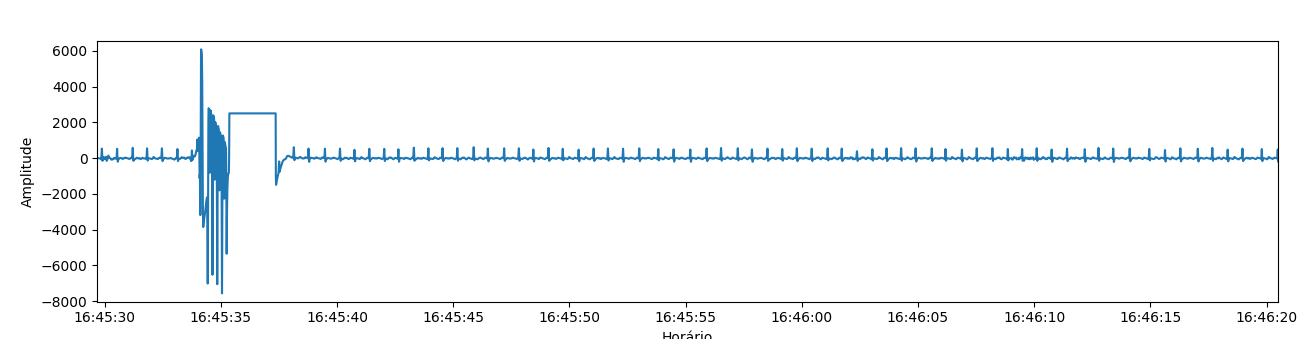
\includegraphics[width=1\linewidth]{imagens/ruido_ecg.png}
    \caption{Ruído gerado no eletrocardiograma do paciente 3 para sincronização dos dados de referência com o vídeo.}
    Fonte: autoria própria.
    \label{fig:ruido-ecg-L8}
\end{figure}

\subsection{Sinal de rPPG}

Os vídeos adquiridos em formato AVI foram utilizados para a extração dos sinais de pulso de volume sanguíneo por meio dos diferentes modelos e algoritmos supervisionados e não supervisionados de rPPG. A partir disso, a comparação da onda de fotopletismografia obtida remotamente com a onda de referência foi realizada por correlação cruzada, de forma a, primeiramente, sincronizar os dois sinais com base no atraso temporal que resulta no maior valor de correlação. Desse modo, foi calculada a correlação de Pearson entre os sinais sincronizados e os resultados para os pacientes 1 e 2 são apresentados na \autoref{tab:rppg_ppg_correlation}, em que os termos entre parênteses representam as bases de dados nas quais foram treinados cada modelo. 

\begin{table*}[h!]
\centering
\caption{Índices de correlação entre os sinais de rPPG e o sinal de PPG de referência para os pacientes 1 e 2.}
\resizebox{0.7\textwidth}{!}{
\begin{tabular}{llcc}
\hline
\textbf{Categoria} & \textbf{Método} & \textbf{Paciente 1} & \textbf{Paciente 2} \\
\hline

\multirow{7}{*}{Não supervisionado}
& CHROM & 0.0991 & 0.5754 \\
& GREEN & \textbf{0.3323} & 0.1350 \\
& ICA   & 0.1114 & 0.6783 \\
& LGI   & 0.1305 & 0.3575 \\
& OMIT  & 0.1336 & 0.3629 \\
& PBV   & 0.1252 & 0.5288 \\
& POS   & 0.1184 & \textbf{0.6884} \\

\hline

\multirow{10}{*}{Supervisionado}
& DeepPhys (PURE) & 0.1070 & 0.4276 \\
& DeepPhys (UBFC) & 0.1061 & 0.4992 \\
& EfficientPhys (PURE) & 0.0944 & 0.4576 \\
& EfficientPhys (UBFC) & 0.0949 & 0.4342 \\
& PhysFormer (PURE) & 0.0740 & 0.4547 \\
& PhysFormer (UBFC) & 0.0602 & 0.4141 \\
& PhysNet (UBFC) & 0.0636 & 0.3151 \\
& PhysNet (PURE) & 0.0425 & 0.4367 \\
& TSCAN (PURE) & 0.1309 & \textbf{0.5650} \\
& TSCAN (UBFC) & \textbf{0.1430} & 0.4505 \\

\hline
\end{tabular}
}
\label{tab:rppg_ppg_correlation}
\end{table*}

Os sinais de rPPG que resultaram no maior coeficiente de correlação entre os métodos supervisionados foram gerados pelo modelo TSCAN treinado no dataset UBFC-rPPG para o paciente 1 e pelo modelo TSCAN treinado no dataset PURE para o paciente 2. Os sinais obtidos por métodos não supervisionados, por sua vez, que resultaram no maior coeficiente de correlação foram obtidos pelo método GREEN para o paciente 1 e pelo método POS para o paciente 2, sendo que esses sinais em comparação com a referência são apresentados na \autoref{fig:corr-waves-examples}. Reitera-se que essa análise não foi realizada para o paciente 3 devido à ausência do sinal de PPG de referência durante a coleta de dados. 

\begin{figure}[h!]
    \centering

    \begin{subfigure}{0.9\linewidth}
        \centering
        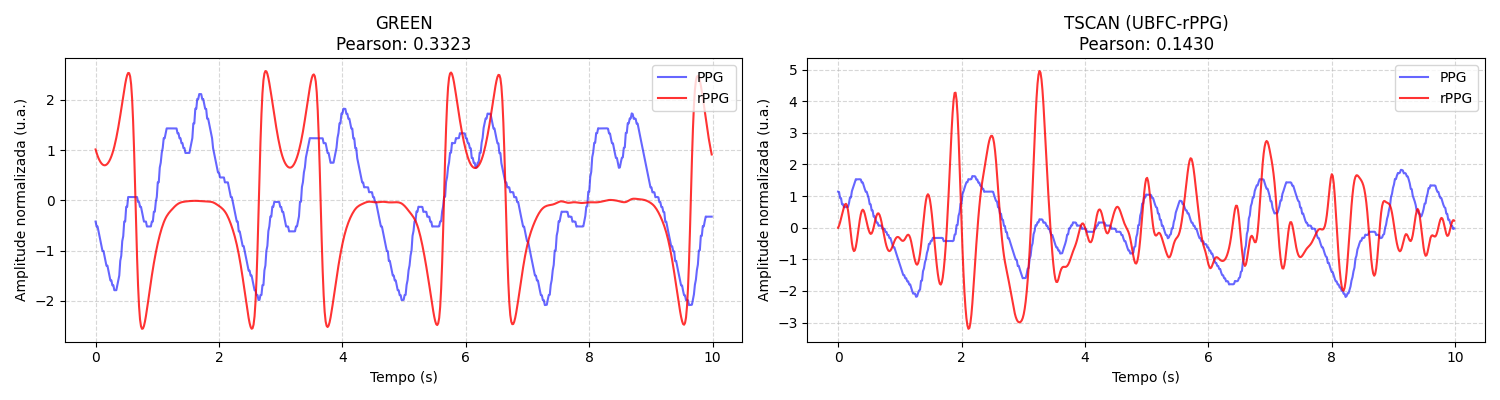
\includegraphics[width=\linewidth]{imagens/corr_examples_L7.png}
        \caption{Paciente 1}
        \label{fig:corr-waves-L7}
    \end{subfigure}

    \vspace{0.2cm}

    \begin{subfigure}{0.9\linewidth}
        \centering
        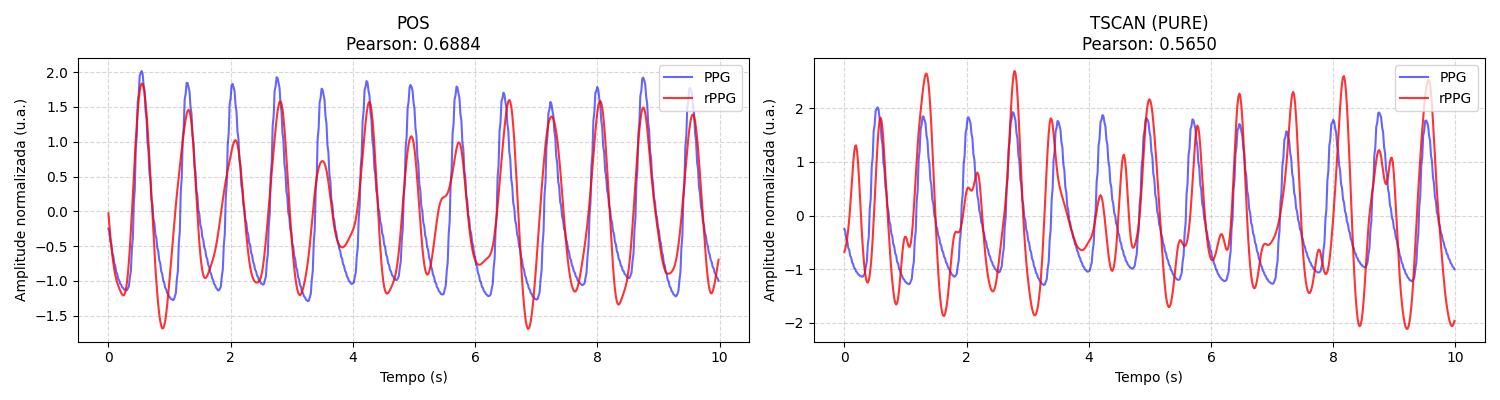
\includegraphics[width=\linewidth]{imagens/corr_examples_L9.png}
        \caption{Paciente 2}
        \label{fig:corr-waves-L9}
    \end{subfigure}

    \caption{Sinais de rPPG dos métodos que obtiveram o maior coeficiente de correlação de Pearson com o sinal de PPG de referência em cada paciente, considerando o alinhamento temporal realizado por meio de correlação cruzada.}
    Fonte: autoria própria.
    \label{fig:corr-waves-examples}

\end{figure}


\subsection{Estimativas de frequência cardíaca}

As estimativas de frequência cardíaca a partir dos sinais gerados por cada método de rPPG foram realizadas considerando o pico do espectro de potência obtido em janelas subsequentes de 15 segundos desses sinais. A partir disso, essas estimativas foram comparadas com as realizadas a partir do sinal de referência de ECG em janelas subsequentes de 15 segundos e foram calculados o erro médio absoluto e o erro médio quadrático em batimentos por minuto, assim como o erro médio percentual. Os resultados referentes aos pacientes 1, 2 e 3 são exibidos na \autoref{tab:rppg_ecg_metrics_all}.


\begin{table*}[htbp]
\centering
\caption{Métricas de erro da estimativa de frequência cardíaca por meio de cada método de rPPG em comparação com as realizadas a partir do ECG para os pacientes 1, 2 e 3.}
\resizebox{\textwidth}{!}{
\begin{tabular}{llcccccccccccc}
\hline
\textbf{Categoria} & \textbf{Método} 
& \multicolumn{4}{c}{\textbf{Paciente 1}} 
& \multicolumn{4}{c}{\textbf{Paciente 2}} 
& \multicolumn{4}{c}{\textbf{Paciente 3}} \\

\cline{3-14}

&
& MAE & RMSE & MAPE & SNR
& MAE & RMSE & MAPE & SNR
& MAE & RMSE & MAPE & SNR \\

\hline

\multirow{7}{*}{Não supervisionado}
& CHROM & \textbf{16.93} & \textbf{19.37} & \textbf{16.12} & -9.80 
& \textbf{0.89} & \textbf{1.06} & \textbf{1.15} & 0.14
& 3.65 & 6.34 & 4.22 & 0.07 \\

& GREEN & 25.89 & 26.13 & 24.75 & \textbf{-9.40}
& 11.60 & 14.99 & 14.93 & -8.39
& 24.60 & 27.50 & 27.02 & -10.80 \\

& ICA & 39.70 & 41.61 & 38.24 & -11.06
& \textbf{0.89} & \textbf{1.06} & \textbf{1.15} & 2.66
& 18.56 & 21.59 & 20.30 & -7.68 \\

& LGI & 26.31 & 26.50 & 25.15 & -9.52
& 4.06 & 5.49 & 5.20 & -3.92
& \textbf{2.59} & \textbf{4.99} & \textbf{3.02} & -2.51 \\

& OMIT & 26.31 & 26.50 & 25.15 & -9.54
& 4.06 & 5.49 & 5.20 & -3.79
& 4.49 & 7.99 & 5.11 & -4.03 \\

& PBV & 26.31 & 26.50 & 25.15 & -9.53
& 1.29 & 1.51 & 1.67 & -0.45
& 2.80 & 5.05 & 3.25 & -1.41 \\

& POS & 28.82 & 34.73 & 27.83 & -9.74
& \textbf{0.89} & \textbf{1.06} & \textbf{1.15} & \textbf{2.83}
& \textbf{2.59} & \textbf{4.99} & \textbf{3.02} & \textbf{1.51} \\

\hline

\multirow{10}{*}{Supervisionado}
& PhysFormer (PURE) 
& \textbf{16.97} & \textbf{26.69} & \textbf{16.43} & \textbf{-6.07}
& 5.68 & 9.53 & 7.21 & -3.85
& 8.25 & 15.92 & 9.08 & -2.56 \\

& PhysFormer (UBFC) 
& 40.54 & 41.43 & 38.67 & -7.96
& 3.09 & 5.87 & 3.91 & -2.61
& 8.53 & 14.37 & 9.42 & -1.96 \\

& EfficientPhys (PURE) 
& 45.47 & 46.69 & 43.43 & -10.40
& 6.44 & 10.87 & 8.18 & -3.10
& 6.82 & 13.82 & 7.52 & \textbf{-0.87} \\

& EfficientPhys (UBFC) 
& 48.49 & 49.84 & 46.33 & -8.49
& 8.27 & 12.05 & 10.52 & -3.72
& 6.82 & 13.82 & 7.52 & -1.61 \\

& PhysNet (PURE) 
& 33.15 & 36.16 & 31.72 & -11.06
& 5.09 & 8.34 & 6.61 & -2.80
& \textbf{1.20} & \textbf{1.87} & \textbf{1.38} & -1.66 \\

& PhysNet (UBFC) 
& 26.20 & 29.30 & 25.10 & -8.59
& 7.78 & 11.48 & 9.89 & -6.01
& 17.86 & 23.15 & 19.59 & -5.36 \\

& TSCAN (PURE) 
& 50.16 & 53.07 & 47.87 & -8.56
& \textbf{1.42} & \textbf{2.05} & \textbf{1.82} & \textbf{-1.25}
& 17.62 & 24.35 & 19.47 & -4.96 \\

& TSCAN (UBFC) 
& 33.15 & 36.16 & 31.72 & -9.69
& 3.93 & 8.05 & 4.96 & -2.87
& 16.61 & 22.73 & 18.59 & -3.96 \\

& DeepPhys (PURE) 
& 51.00 & 51.35 & 48.77 & -11.68
& 13.56 & 19.26 & 17.37 & -3.50
& 29.52 & 34.72 & 32.99 & -6.25 \\

& DeepPhys (UBFC) 
& 50.16 & 51.83 & 47.81 & -10.24
& 10.79 & 16.05 & 13.74 & -2.71
& 18.72 & 25.62 & 21.06 & -3.07 \\

\hline
\end{tabular}
}
\label{tab:rppg_ecg_metrics_all}
\end{table*}

É possível observar que o método não supervisionado que resultou no menor valor de erro absoluto médio para o paciente 1 foi o método CHROM. Em relação ao sinal do paciente 2, os métodos CHROM, ICA e POS resultaram nos menores valores de erro comparados ao restante dos métodos. Além disso, os métodos LGI e POS foram os que resultaram nos menores valores de erro para as estimativas de frequência cardíaca a partir dos sinais do paciente 3. No que se refere aos métodos supervisionados, por sua vez, o modelo PhysFormer treinado do dataset PURE foi o que apresentou o melhor resultado para o paciente 1, o modelo TSCAN treinado no dataset PURE resultou no menor valor de erro para as estimativas do paciente 2 e o modelo PhysNet treinado no mesmo dataset foi o que obteve o melhor resultado para o paciente 3. À parte isso, a comparação entre todos os métodos permite analisar que o método POS foi o que resultou na melhor relação sinal-ruído para os sinais dos pacientes 2 e 3. Já para o paciente 1, o sinal gerado pelo modelo PhysFormer treinado na base de dados PURE foi o que apresentou o melhor valor para essa métrica.

Observa-se, por fim, que os métodos CHROM, ICA e POS aplicados ao sinal do paciente 2 resultaram no menor valor de erro absoluto médio entre todos os algoritmos não supervisionados. Da mesma forma, o modelo TSCAN treinado no dataset PURE também aplicado ao sinal do paciente 2 resultou no menor erro absoluto médio entre os modelos supervisionados. Na \autoref{fig:best-specs-L9}, pode-se analisar os espectrogramas de dois desses sinais, a partir dos quais é possível identificar a região da frequência de maior densidade de potência de forma distinguível ao longo de toda a duração do sinal. 

\begin{figure}[h!]
    \centering
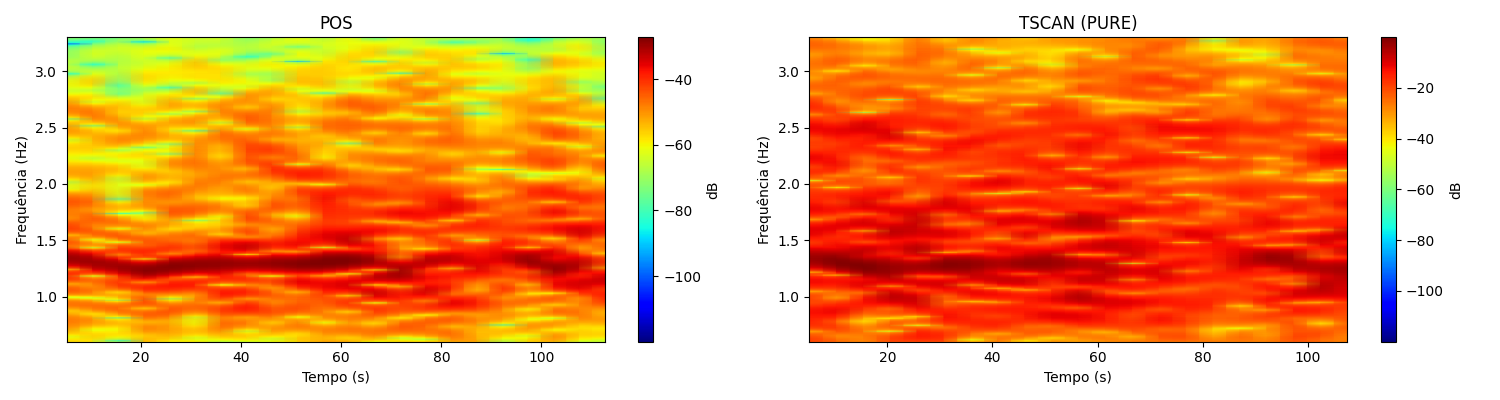
\includegraphics[width=1\linewidth]{imagens/best_specs_L9.png}
    \caption{Espectrogramas de dois dos sinais de rPPG cujas estimativas de frequência cardíaca resultaram no menor erro absoluto médio em relação às estimativas obtidas por meio do ECG.}
    Fonte: autoria própria
    \label{fig:best-specs-L9}
\end{figure}

Similarmente, os espectros de potência desses sinais apresentados na \autoref{fig:best-psd-L9} permitem a identificação do pico referente à essa frequência, a partir da qual pode ser realizada a estimativa do valor de frequência cardíaca. Nesse caso, a análise em frequência foi realizada no sinal completo com duração próxima a dois minutos. Em comparação, as estimativas de frequência cardíaca por janela são apresentadas na \autoref{fig:best-estimates-L9}. 


\begin{figure}[h!]
    \centering
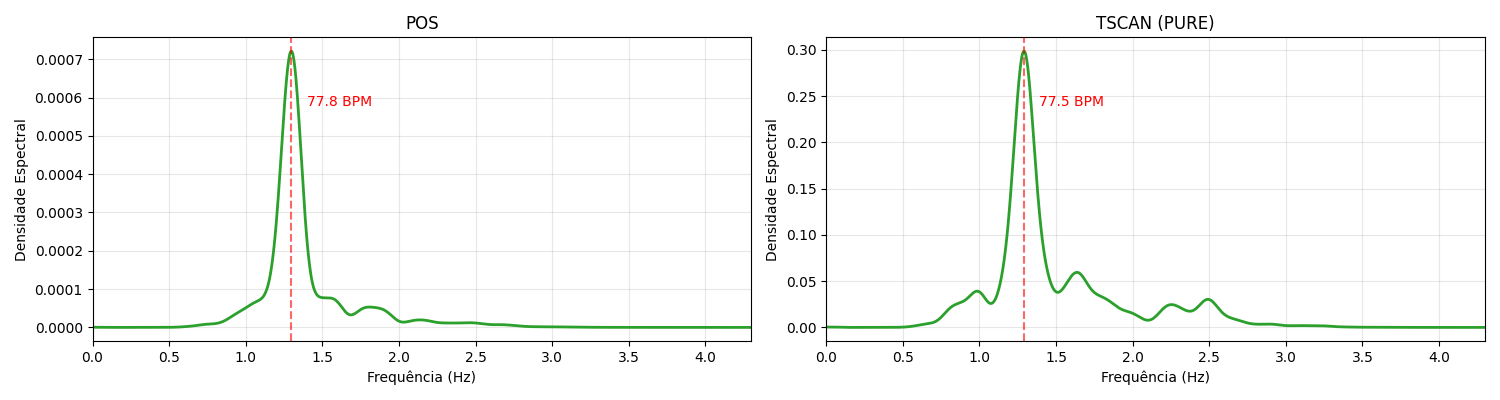
\includegraphics[width=1\linewidth]{imagens/best_psds_L9.png}
    \caption{Espectros de potência de dois dos sinais de rPPG cujas estimativas de frequência cardíaca resultaram no menor erro absoluto médio em relação às estimativas obtidas por meio do ECG}
    Fonte: autoria própria
    \label{fig:best-psd-L9}
\end{figure}

\begin{figure}[h!]
    \centering
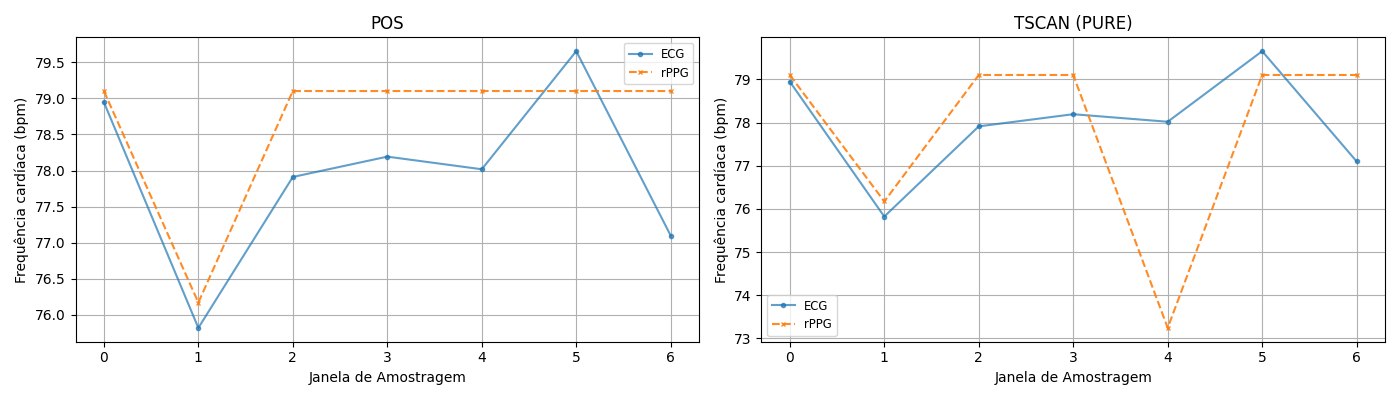
\includegraphics[width=1\linewidth]{imagens/best_estimates_L9.png}
    \caption{Estimativas de frequência cardíaca por janela obtidas por meio de dois dos métodos de rPPG que resultaram no menor erro absoluto médio em relação às estimativas obtidas por meio do ECG}
    Fonte: autoria própria
    \label{fig:best-estimates-L9}
\end{figure}

Ademais, é possível observar o erro absoluto médio entre todos os métodos não supervisionados em comparação com os métodos supervisionados em cada janela para os pacientes 1 e 2 na \autoref{fig:mean-error-per-window-preliminar}. Verifica-se que, para cada paciente, os dois tipos de métodos possuem alguns picos de erro em comum, a exemplo da janela 5 do sinal do paciente 2, que representa o maior erro para ambos os tipos de algoritmo. De forma análoga, a janela de índice zero desse sinal é a que resulta no menor erro absoluto médio para os dois tipos de método.

\begin{figure}[h!]
    \centering
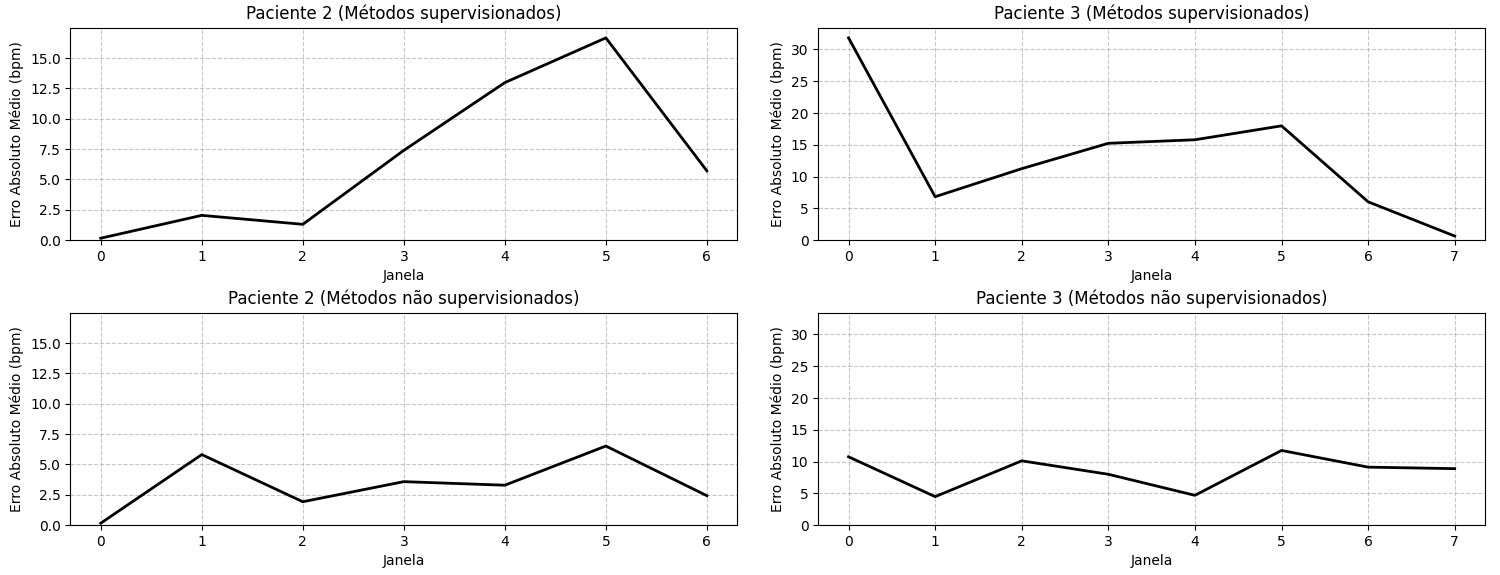
\includegraphics[width=1\linewidth]{imagens/mean_error_per_window_2e3.png}
    \caption{Erro absoluto médio por janela das estimativas de frequência cardíaca realizadas a partir dos métodos supervisionados e não supervisionados para os pacientes 2 e 3.}
    Fonte: autoria própria
    \label{fig:mean-error-per-window-preliminar}
\end{figure}


% \clearpage
\section{Coleta de validação}

Na coleta de validação, foram extraídos dois vídeos de um indivíduo saudável e os sinais de eletrocardiograma correspondentes. No primeiro vídeo coletado, o indivíduo apresentou pouca movimentação, enquanto no vídeo subsequente houve maior movimentação do rosto causada por fala, riso e rotações sutis da cabeça.

\subsection{Sincronização dos dados}

A sincronização entre os dados de vídeo e o sinal de referência foi realizada por meio da geração de um ruído no ECG devido a um impacto no eletrodo utilizado. Esse impacto é visível no sinal, conforme demonstra a \autoref{fig:ruido-ecg-valid}, sendo que foi considerado o sinal 5 segundos após o pico observado. Da mesma forma, são considerados os quadros do vídeo a partir de 5 segundos após o primeiro quadro em que é identificada a interferência no eletrodo.

\begin{figure}[h!]
    \centering
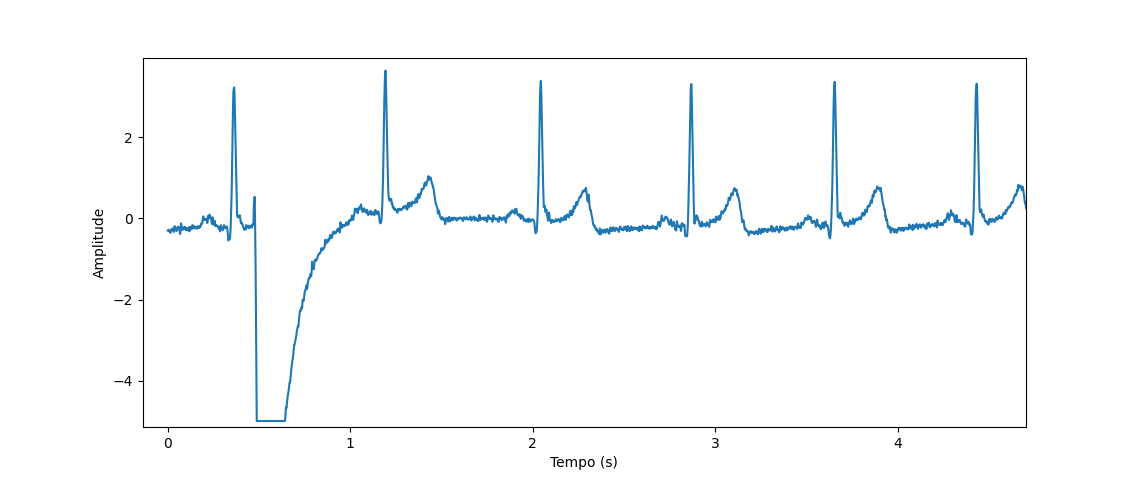
\includegraphics[width=0.7\linewidth]{imagens/ruido_ecg_valid.png}
    \caption{Exemplo do ruído gerado no eletrocardiograma para sincronização de dados da coleta de validação}
    Fonte: autoria própria
    \label{fig:ruido-ecg-valid}
\end{figure}

\subsection{Estimativas de frequência cardíaca}

% \begin{figure}[h!]
%     \centering
% 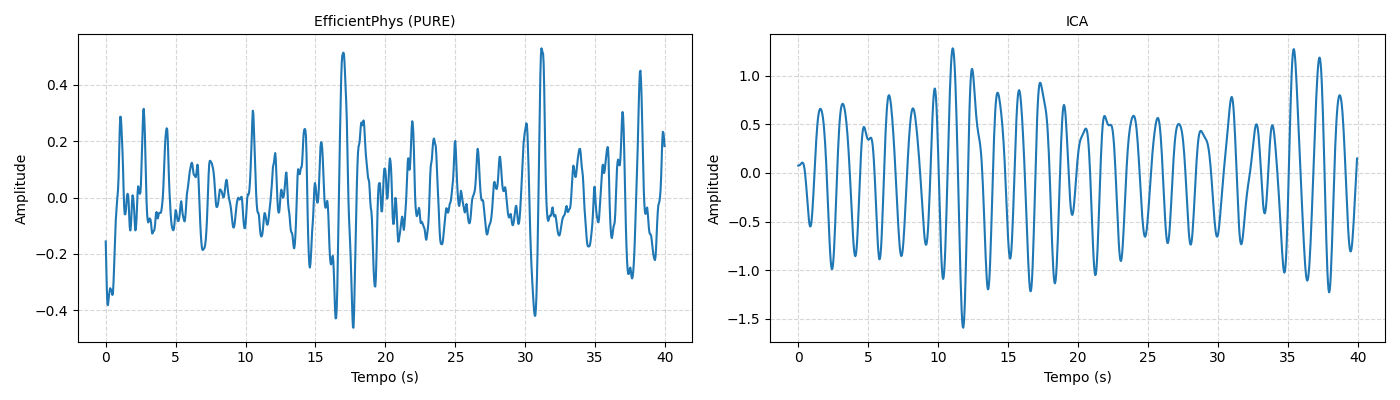
\includegraphics[width=1\linewidth]{imagens/waves_examples.png}
%     \caption{Exemplos de sinais resultantes extraídos a partir do primeiro vídeo da coleta de validação}
%     Fonte: autoria própria
%     \label{fig:waves-valid}
% \end{figure}

A partir dos sinais de pulso de volume sanguíneo obtidos por meio de cada um dos métodos e modelos de fotopletismografia remota aplicados aos dois vídeos adquiridos durante a coleta de validação, foram realizadas as estimativas de frequência cardíaca por meio da análise espectral desses sinais baseada na Transformada Rápida de Fourier em janelas subsequentes de 15 segundos. Essas estimativas foram comparadas com as obtidas a partir do ECG também em janelas subsequentes de 15 segundos. Os resultados dessas comparações são dispostos na \autoref{tab:rppg_ecg_metrics_valid}. 

\begin{table*}[h!]
\centering
\caption{Métricas de erro das estimativas de frequência cardíaca por meio de cada método de rPPG em comparação com as realizadas a partir do ECG para os vídeos 1 e 2.}
\resizebox{\textwidth}{!}{
\begin{tabular}{llcccccccc}
\hline
\textbf{Categoria} & \textbf{Método} 
& \multicolumn{4}{c}{\textbf{Vídeo 1}} 
& \multicolumn{4}{c}{\textbf{Vídeo 2}} \\
\cline{3-6} \cline{7-10}
& 
& \textbf{MAE} & \textbf{RMSE} & \textbf{MAPE} & \textbf{SNR} 
& \textbf{MAE} & \textbf{RMSE} & \textbf{MAPE} & \textbf{SNR} \\
\hline

\multirow{7}{*}{Não supervisionado}
& CHROM & 3.11 & 4.67 & 4.23 & 0.71 
         & 7.30 & 8.42 & 9.05 & \textbf{-5.40} \\

& GREEN & 8.85 & 11.73 & 12.18 & -6.40 
         & 7.59 & 9.03 & 9.71 & -8.42 \\

& ICA   & \textbf{1.69} & \textbf{2.25} & \textbf{2.32} & \textbf{4.74} 
         & 10.94 & 12.55 & 13.81 & -7.06 \\

& LGI   & 1.86 & 2.35 & 2.56 & 0.39 
         & \textbf{5.86} & \textbf{7.39} & \textbf{7.40} & -6.81 \\

& OMIT  & 1.86 & 2.35 & 2.56 & 0.21 
         & \textbf{5.86} & \textbf{7.39} & \textbf{7.40} & -6.75 \\

& PBV   & 2.03 & 2.46 & 2.79 & -2.44 
         & 6.98 & 7.74 & 8.63 & -7.94 \\

& POS   & 1.86 & 2.35 & 2.56 & 1.49 
         & 9.97 & 12.77 & 12.52 & -5.84 \\

\hline

\multirow{10}{*}{Supervisionado}

& PhysFormer (PURE) & 2.34 & 3.43 & 3.23 & -3.66 
                     & 12.67 & 16.13 & 15.56 & \textbf{-5.62} \\

& PhysFormer (UBFC) & 57.39 & 59.45 & 79.59 & -5.64 
                     & 32.36 & 36.73 & 41.80 & -7.68 \\

& EfficientPhys (PURE) & \textbf{1.69} & \textbf{2.25} & \textbf{2.32} & \textbf{-0.96} 
                        & \textbf{10.40} & \textbf{12.81} & \textbf{12.68} & -7.59 \\

& EfficientPhys (UBFC) & 5.58 & 8.14 & 7.71 & -2.99 
                       & 11.58 & 14.86 & 14.16 & -6.23 \\

& PhysNet (PURE) & 5.08 & 9.01 & 7.00 & -2.33 
                  & 11.09 & 16.73 & 13.90 & -6.40 \\

& PhysNet (UBFC) & 40.79 & 43.55 & 56.31 & -8.38 
                  & 39.06 & 40.00 & 50.00 & -9.31 \\

& TSCAN (PURE) & 3.64 & 4.96 & 5.02 & -2.71 
                & 11.09 & 15.57 & 13.42 & -6.47 \\

& TSCAN (UBFC) & 13.29 & 20.32 & 18.13 & -6.05 
                & 24.31 & 26.52 & 30.95 & -7.56 \\

& DeepPhys (PURE) & 13.27 & 16.11 & 18.39 & -5.56 
                   & 18.68 & 20.76 & 23.77 & -7.10 \\

& DeepPhys (UBFC) & 9.49 & 11.02 & 13.01 & -6.09 
                   & 16.01 & 20.10 & 20.28 & -6.70 \\

\hline
\end{tabular}
}
\label{tab:rppg_ecg_metrics_valid}
\end{table*}


Pode-se verificar que, entre os métodos não supervisionados, o método ICA foi o que resultou em estimativas de frequência cardíaca com o menor erro 
médio absoluto para o vídeo 1 e os métodos LGI e OMIT resultaram no menor erro para o vídeo 2. Em relação aos modelos supervisionados, o modelo EfficientPhys 
treinado na base de dados PURE foi o que apresentou o menor erro médio absoluto em ambos os vídeos. Ademais, o método ICA foi o que resultou, entre todos os métodos, 
no melhor valor de SNR para o vídeo 1, enquanto o método CHROM foi o que gerou o melhor valor para o vídeo 2. 

Por fim, entre todos os métodos avaliados em ambos os vídeos, o método ICA e o modelo EfficientPhys treinado na base PURE aplicados ao sinal do vídeo 1 
foram os que apresentaram os menores valores de erro médio absoluto. Os espectrogramas referentes aos sinais resultantes desses algoritmos são apresentados 
na \autoref{fig:specs-valid}, bem como seus respectivos espectros de potência na \autoref{fig:best-psd-valid}. A partir das figuras, observa-se que a 
frequência com maior densidade de potência pode ser identificada de forma distinguível, a partir da qual pode ser realizada a estimativa de frequência cardíaca. 
Nesse caso, a análise espectral foi realizada no sinal em sua completude. Complementarmente, as estimativas de frequência cardíaca realizadas por janela são 
dispostas na \autoref{fig:best-estimates-valid}.

\begin{figure}[h!]
    \centering
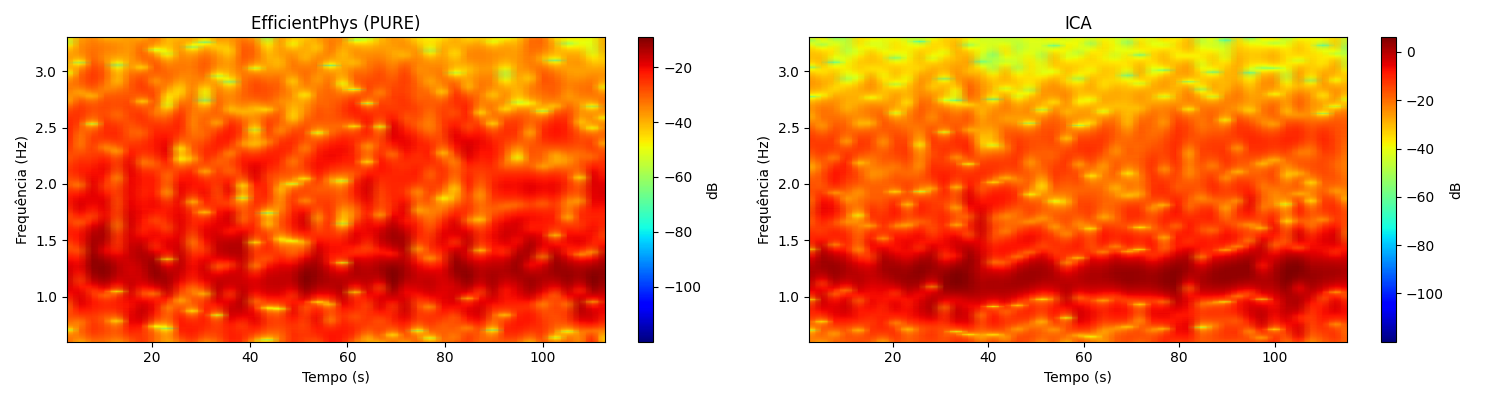
\includegraphics[width=1\linewidth]{imagens/best_specs_valid.png}
    \caption{Espectrogramas dos sinais cujas estimativas de frequência cardíaca resultaram no menor erro médio absoluto.}
    Fonte: autoria própria
    \label{fig:specs-valid}
\end{figure}

\begin{figure}[h!]
    \centering
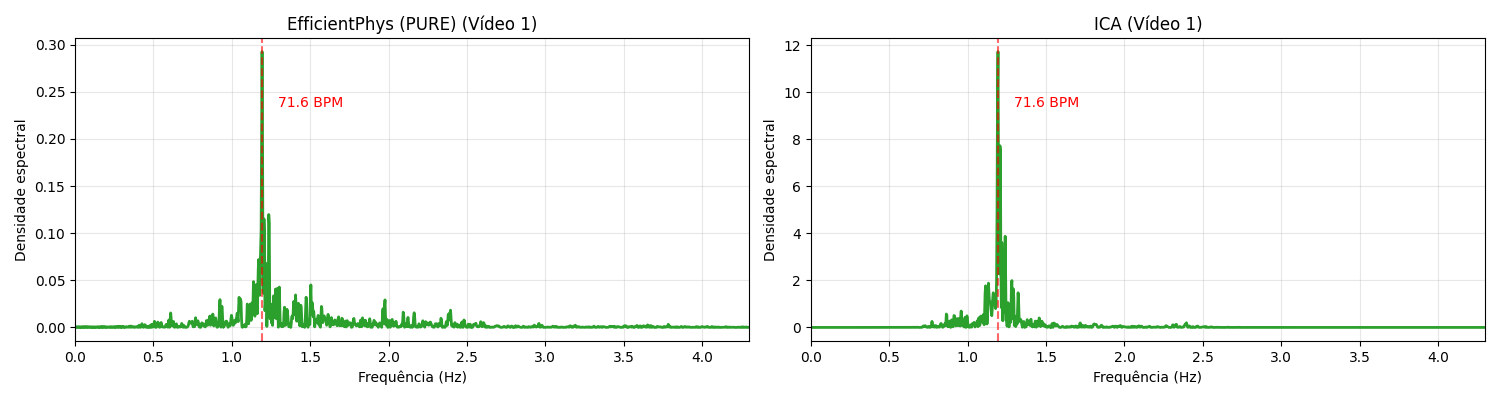
\includegraphics[width=1\linewidth]{imagens/best_psd_valid.png}
    \caption{Espectros de potência dos sinais cujas estimativas de frequência cardíaca resultaram no menor erro médio absoluto.}
    Fonte: autoria própria
    \label{fig:best-psd-valid}
\end{figure}

\begin{figure}[h!]
    \centering
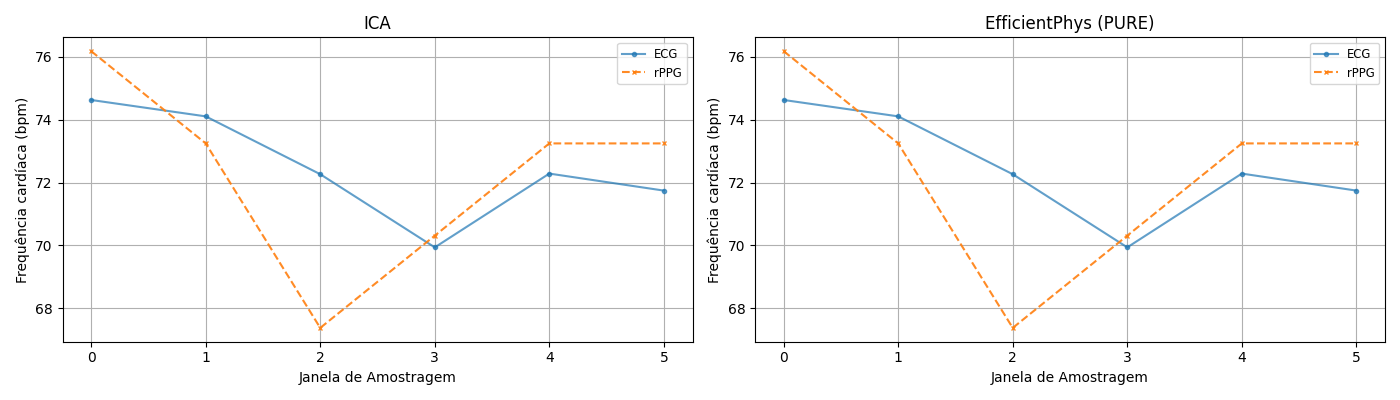
\includegraphics[width=1\linewidth]{imagens/best_estimates_valid.png}
    \caption{Estimativas de frequência cardíaca por janela dos sinais que resultaram no menor erro médio absoluto.}
    Fonte: autoria própria
    \label{fig:best-estimates-valid}
\end{figure}

Ademais, são apresentadas as curvas de erro absoluto médio dos métodos não supervisionados em comparação com os métodos supervisionados para os dois vídeos na \autoref{fig:mean-error-window-valid}. Pode-se observar como essas curvas de erro exibem comportamentos temporalmente semelhantes entre os dois grupos de métodos, com ocorrências coincidentes de aumento e redução do erro em múltiplas janelas consecutivas.

\begin{figure}[h!]
    \centering
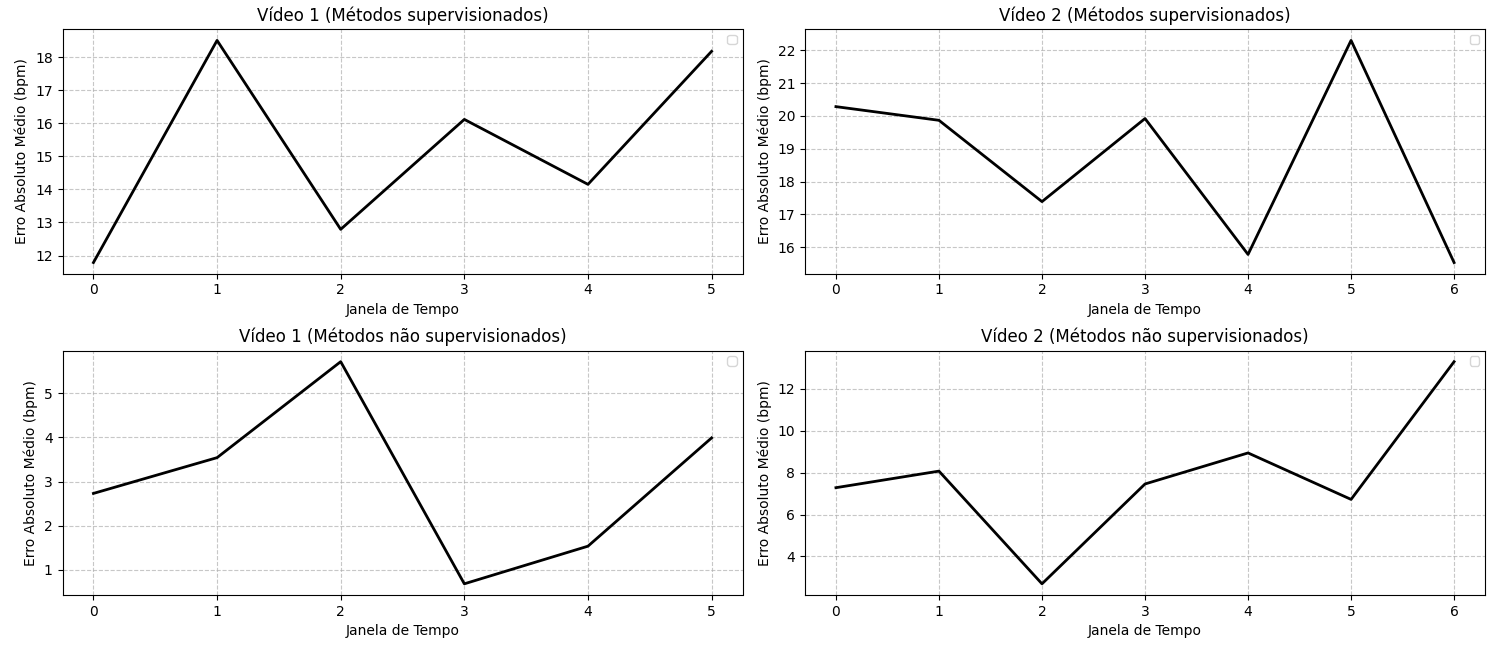
\includegraphics[width=1\linewidth]{imagens/mean_error_per_window_valid.png}
    \caption{Erro absoluto médio por janela dos métodos supervisionados e não supervisionados de cada vídeo da coleta de validação.}
    Fonte: autoria própria
    \label{fig:mean-error-window-valid}
\end{figure}
	

\newpage\chapter{Discussão preliminar}

Com base no que foi disposto, verifica-se que a extração de sinais de fotopletismografia remota a partir de vídeos de pacientes internados em Unidades de Terapia Intensiva pode ser realizada por meio de métodos baseados em algoritmos e modelos matemáticos, denominados métodos não supervisionados, bem como pode ser realizada por meio de modelos baseados em aprendizado profundo, referidos como métodos supervisionados. Esses métodos resultam em uma onda de pulso de volume sanguíneo a qual possui  correspondência identificável com o sinal de fotopletismografia convencional e a partir da qual podem ser estimados valores de frequência cardíaca e de frequência respiratória. No entanto,  artefatos de iluminação e de movimento impactam de forma significativa na qualidade do sinal extraído, como foi possível verificar a partir dos resultados da Coleta Preliminar 2, na qual as estimativas de frequência cardíaca extraídas do vídeo com maior incidência desses elementos apresentaram, para a maioria dos métodos analisados, maior erro médio absoluto em relação aos valores de referência obtidos por meio do eletrocardiograma, quando comparado às estimativas advindas do vídeo em que o indivíduo monitorado permaneceu imóvel. De maneira complementar, a análise do erro médio por janela das estimativas de frequência cardíaca realizada tanto nos dados da Coleta Preliminar 1, quanto nos dados da Coleta Preliminar 2, permite identificar valores maiores de erro em janelas nas quais há mudanças expressivas de iluminação ou da posição do rosto, o que reforça o impacto desses artefatos. Além disso, artefatos de compressão de imagem também impactam negativamente no sinal de rPPG extraído, por isso a aquisição de dados foi realizada com a utilização de uma câmera industrial, com o intuito de minimizar a influência desse fator.

Ademais, o sinal que pode ser obtido por métodos de fotopletismografia remota é influenciado pela detecção e rastreamento da região de interesse, o que foi verificado no processamento dos dados da Coleta Preliminar 1. Nesse caso, o sinal extraído a partir do vídeo do paciente 1 apresentou um baixo índice de correlação com o sinal de fotopletismografia de referência, bem como as estimativas de frequência cardíaca realizadas resultaram nos maiores valores de erro médio absoluto entre todos os resultados. Isso pode ser explicado devido ao fato de que a ferramenta de detecção de face utilizada não reconheceu o rosto do paciente, similar a situações descritas por \citeonline{van2025camera} em relação ao monitoramento remoto em UTI, possivelmente devido à oclusão significativa dessa região, em decorrência da presença de equipamentos de suporte ventilatório. Assim, para todos os métodos, foram utilizados os quadros completos do vídeo como entrada, o que gera o aumento da incidência de elementos de ruído e, consequentemente, a degradação do sinal, o que é atenuado quando apenas a região de interesse é introduzida aos modelos. Observa-se, ainda, que nesse caso o sinal de PPG de referência difere da forma de onda fotopletismográfica convencional esperada, o que pode decorrer de fatores fisiológicos relacionados à condição clínica do paciente, de modo que são necessárias análises mais aprofundadas para esclarecer esse tipo de influência sobre o sinal obtido remotamente.

No que se refere às estimativas de frequência respiratória, nota-se que o sinal respiratório de referência do paciente 3 apresentou ruído de forma que o espectro de potência respectivo a esse sinal possui um espalhamento na banda de interesse e não possui um único pico distinguível (vide Apêndice \ref{apendice:spec-freqresp}). Nesse sentido, a ausência de um pico espectral dominante dificulta a definição inequívoca da frequência respiratória de referência, de modo que parte da discrepância observada entre as estimativas e a referência, nesse caso, pode estar associada à própria qualidade do sinal de referência, e não exclusivamente ao desempenho dos métodos avaliados.

Por fim, a partir dos valores de erro médio absoluto para as estimativas de frequência cardíaca e para as estimativas de frequência respiratória tanto a partir dos dados da Coleta Preliminar 1 quanto da Coleta Preliminar 2, nota-se que os métodos supervisionados apresentaram resultados comparáveis aos métodos não supervisionados, apesar de demandarem maior custo computacional para inferência. Ademais, entre os métodos supervisionados, modelos de mesma estrutura treinados em bases de dados diferentes resultaram em estimativas com erros expressivamente diferentes em relação à referência, o que demonstra a influência do conjunto de dados de treinamento no desempenho dos modelos em situações realistas. Por conseguinte, ambos os tipos de método de extração de sinais de fotopletismografia remota apresentam métricas de erro e valores para a razão sinal-ruído que reafirmam o potencial de aplicação desse tipo de tecnologia em situações clínicas. Faz-se necessário, todavia, a análise em uma quantidade maior de amostras para que conclusões mais detalhadas possam ser esclarecidas. 



% \newpage\input{paginas/conclusao}
	
%\chapter{Capítulo com epígrafe}
%\capepigrafe[0.5\textwidth]{``Frase espirituosa de um autor famoso''}{Autor famoso}


% ========== Referências ==========
% --- IEEE ---
%	http://www.ctan.org/tex-archive/macros/latex/contrib/IEEEtran
%\bibliographystyle{IEEEbib}

% --- ABNT (requer ABNTeX 2) ---
%	http://www.ctan.org/tex-archive/macros/latex/contrib/abntex2
%\bibliographystyle{abntex2-num}


% ========== Apêndices (opcional) ==========
\newpage
\apendice
\chapter{ESPECTRO DE POTÊNCIA DE SINAL RESPIRATÓRIO COM MÚLTIPLOS PICOS DOMINANTES}
\label{apendice:spec-freqresp}
%\blindtext

\begin{figure}[h!]
    \centering
    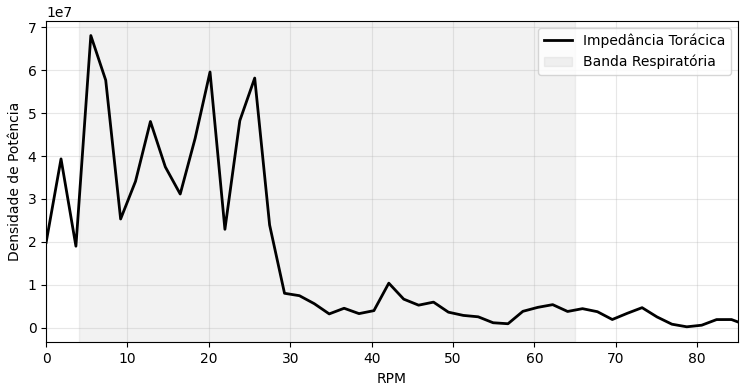
\includegraphics[width=1\linewidth]{imagens/ref_spec_L8.png}
    \caption{Espectro de potência do sinal respiratório de referência do paciente 3. Nota-se o espalhamento na banda de potência e a identificação de mais de um pico distinguível.}
    Fonte: autoria própria
    \label{fig:ref_spec_L8}
\end{figure}

\newpage

% \newpage
%\chapter{Beta}
% ========== Anexos (opcional) ==========
% \anexo
% \newpage\input{paginas/anexo}
\newpage
\referencias
\bibliography{bib/mybib}
\end{document}